\documentclass{scrartcl}

\title{Kommunikationssysteme Selbstlernfragen und Antworten}
\author{Sven Bergmann}
\date{\today}

% !TeX root = main.tex


\usepackage[ngerman]{babel}
\usepackage[T1]{fontenc}
\usepackage{lmodern}
\usepackage[utf8]{inputenc}
\usepackage{natbib}
\usepackage{graphicx}
\usepackage[colorinlistoftodos,prependcaption,textsize=tiny]{todonotes}
\usepackage{listingsutf8}
\usepackage{microtype}
\usepackage[shortlabels]{enumitem}
\usepackage{tabularx}
\usepackage{amsmath}
\usepackage{xcolor}
\usepackage{listings}
\usepackage{mathtools}
\usepackage{hyperref}

\inputencoding{utf8}


\hypersetup{
    pdftitle = {Kommunikationssysteme Selbstlernfragen und Antworten},
    pdfauthor = {Sven Bergmann},
    pdfsubject = {Kommunikationssysteme},
    pdfkeywords = {Kommunikationssysteme, Selbstlernfragen, Antworten}
}

\begin{document}

    \maketitle

    \tableofcontents

    \addsec{Vorlesung 1 - Schichtenmodelle}

\minisec{Was ist der Unterschied zwischen Client-Server und Peer-to-Peer Netzwerken?}
\begin{itemize}
    \item \textcolor{blue}{Client-Server}
    \begin{itemize}
        \item Server-Prozess: Langlebige Anwendung, die kontinuierlich auf Anfragen wartet, diese verarbeitet und beantwortet
        \item Client-Prozess: Zumeist kurzlebige Anwendung die Anfragen an den Server-Prozess stellt und auf die Antwort wartet.
        Die Rolle ist damit zumeist beendet
    \end{itemize}
    \item \textcolor{blue}{Peer-to-Peer}
    \begin{itemize}
        \item Gleichrangige Kommunikationspartner
        \item Oft bessere Leistung als Client-Server
        \item Übergreifender Datenbestand
    \end{itemize}
\end{itemize}

\minisec{Welche Arten Proxies existieren in Rechnernetzen, und welche Aufgaben haben sie typischerweise?}
\begin{itemize}
    \item Forward Proxy
    \item Reverse Proxy
    \item Aufgaben:
    \begin{itemize}
        \item Proxy zum Zwischenspeichern/Anonymisieren
        \item Proxy zum Lastbalancieren von Webseiten
    \end{itemize}
\end{itemize}

\minisec{Wie unterscheiden sich Point-to-Point und Multi-Access-Netzwerke?}
\begin{itemize}
    \item \textcolor{blue}{Point-to-Point (Punkt-zu-Punkt)}
    \begin{itemize}
        \item Ein Paar von Rechnern ist durch eine direkte Leitung verbunden
        \item kein anderer Rechner kann diese Leitung nutzen
        \item Full-Duplex: Senden und Empfangen gleichzeitig möglich
        \item Half-Duplex: Nur eines von beiden gleichzeitig möglich
        \item Simplex: Daten können nur in eine Richtung fließen
    \end{itemize}
    \item \textcolor{blue}{Multi-Access-Netze}
    \begin{itemize}
        \item Mehrere angeschlossenen Rechner teilen sich einen Übertragungskanal
        \item Damit Daten trotzdem an den richtigen Empfänger gesendet werden, müssen sie mit einer Zieladresse versehen werden
        \item Daten werden in Übertragungseinheiten (Frames) eingeteilt und mit der Adresse des Empfängers ausgewiesen
        \item „Rechner“ prüfen, ob die Nachricht für sie ist (aktiver Vorgang!)
        \item Sollen alle Stationen gleichzeitig eine Nachricht erhalten, so werden Broadcast-Adressen (spezielle Adressen zur Adressierung aller Stationen) verwendet
    \end{itemize}
\end{itemize}

\minisec{Welche Konsequenzen entstehen für die Datenkommunikation im Falle von Multi-Access-Netzwerken?}
\begin{itemize}
    \item Mehrere angeschlossenen Rechner teilen sich einen Übertragungskanal
    \item Damit Daten trotzdem an den richtigen Empfänger gesendet werden, müssen sie mit einer Zieladresse versehen werden
    \item Daten werden in Übertragungseinheiten (Frames) eingeteilt und mit der Adresse des Empfängers ausgewiesen
    \item „Rechner“ prüfen, ob die Nachricht für sie ist (aktiver Vorgang!)
    \item Sollen alle Stationen gleichzeitig eine Nachricht erhalten, so werden Broadcast-Adressen (spezielle Adressen zur Adressierung aller Stationen) verwendet
\end{itemize}

\minisec{Wie unterscheiden sich statische und dynamische Netzwerke?}
\begin{itemize}
    \item \textcolor{blue}{Statische Netze:}
    \begin{itemize}
        \item fest verdrahtete Punkt-zu-Punkt Verbindungen oder Multi-Access-Netze
        \item jeder Knoten besitzt eine feste Anzahl von Nachbarn oder einen Zugang zu einem Multi-Access-Netze
        \item besitzen keine inhärent im Netz verankerte Vermittlungsfunktion
        \item Vermittlung über Netzgrenzen hinweg jedoch durch Weiterleiten möglich (Store-and-Forward)
    \end{itemize}
    \item \textcolor{blue}{Dynamische Netze:}
    \begin{itemize}
        \item Verbindungen enthalten konfigurierbare Schaltelemente
        \item diese können dynamisch vermitteln (Weg wird geschaltet)
        \item ein- oder mehrstufiger Aufbau möglich
        \item Mit Aufwand blockadefreie Schaltungen ohne Crossbar
    \end{itemize}
\end{itemize}

\minisec{Ordnen Sie die Begriffe Paketvermittlung und Leitungsvermittlung zu!}
\begin{itemize}
    \item Die \textcolor{blue}{Leitungsvermittlung (circuit switching} stellt zwischen zwei oder mehr Teilnehmern einen Übertragungskanal über mehrere Vermittlungsstellen für die Dauer der Übertragung her.
    Die Leitungsvermittlung eignet sich in der Regel für zeitkritische Anwendungen bzw.\ der Übertragung von Daten in Echtzeit.
    \item Bei der  \textcolor{blue}{Paketvermittlung (store and forward} werden die Daten oder Informationen in Pakete aufgeteilt.
    Der Dienst bzw.\ die Anwendung übergibt die einzelnen Pakete an das Kommunikationssystem und versieht sie mit der Zieladresse und weiteren Vermittlungsinformationen.
    Das Kommunikationssystem vermittelt die Datenpakete vom Sender zum Empfänger.
    Die Pakete können dabei unterschiedliche Wege zu ihrem Ziel nehmen.
    Beim Empfänger werden die Datenpakete dann wieder zusammengesetzt.
    Die Paketvermittlung eignet sich für zeitunkritische Übertragungen.
\end{itemize}

\minisec{Was versteht man unter dem Store-and-Forward-Verfahren, und wo wird es eingesetzt?}
\begin{itemize}
    \item Im Netze findet ein Store-and-Forward statt.
    An der Grenze zwischen zwei Netzen sorgen Router für die Weiterleitung der Daten.
    Nach dem Empfang findet die Entscheidung über den nächsten Router konzeptionell anhand der Zieladresse statt.
    \item Wird in der Internet-Schicht eingesetzt (entspricht ISO/OSI 3) bei statischen Netzen
\end{itemize}

\minisec{Welche Metriken kennen Sie, um Topologien von Rechnernetzen zu charakterisieren?}
\begin{itemize}
    \item \textcolor{blue}{Durchmesser (Diameter)}
    \begin{itemize}
        \item Maximaler Abstand zweier Knoten, d.\ h. die Anzahl von Kanten
        \item → Ziel: Möglichst klein (Zeitbedarf für Übertragung)
    \end{itemize}
    \item \textcolor{blue}{Bisektionsbreite (Connectivity)}
    \begin{itemize}
        \item Minimale Anzahl von Kanten die man entfernen muss, um das Netzwerk in zwei Hälften zu teilen
        \item → Ziel: Möglichst groß zur Verbesserung der Fehlertoleranz
    \end{itemize}
    \item \textcolor{blue}{Knotengrad}
    \begin{itemize}
        \item Anzahl von Verbindungen eines Knotens zu seinen Nachbarn.
        Ist die Anzahl nicht konstant, so wird der das Maximum aller Knoten genommen
        \item → Ziel: Möglichst klein, da die Kosten so mit diesem Grad steigen
    \end{itemize}
\end{itemize}

\minisec{ Welche räumliche Ausdehnung besitzen typischerweise LANs?}
\begin{itemize}
    \item 10 m – wenige km
\end{itemize}

\minisec{Was versteht man unter einem Protokoll im Kontext der Datenkommunikation?}
\begin{itemize}
    \item \textcolor{blue}{Ein Protokoll ist die Gesamtheit aller Vereinbarungen zwischen Computeranwendungen zum Zweck einer gemeinsamen Kommunikation}
\end{itemize}

\minisec{Nennen Sie 3--4 Problemdomänen, die für eine erfolgreiche Datenkommunikation zu lösen sind!}
\begin{itemize}
    \item \todo 1 3–4 Problemdomänen nennen
\end{itemize}

\minisec{Welche Vorteile (und ggf. auch Nachteile) haben Schichten-Architekturen?}
\begin{itemize}
    \item Vorteile:
    \begin{itemize}
        \item Einzelne Schichten sind leicht veränderbar, bei der Einhaltung der Schnittstellen/Interfaces
        \item Bei Veränderung der Schnittstellen/Interfaces sind nur die beiden angrenzenden Schichten betroffen
        \item Schichtenarchitekturen kapseln Maschinenabhängigkeiten, daher leicht portierbar.
        Nur die innerste Schicht muss neu implementiert werden
    \end{itemize}
    \item Nachteile:
    \begin{itemize}
        \item Es ist schwierig Systeme sauber in Schichten zu strukturieren.
        Wenn äußere Schichte Dienste der inneren Schichten benötigen, wird leicht die einfache Abhängigkeit von der nächst unteren Schicht zerstört
        \item Es kann Performanz-Probleme geben, weil mit dem Zugriff auf die Dienste eine Schicht immer eine gewisser Overhead verbunden ist
    \end{itemize}
\end{itemize}

\minisec{Wie heißen die sieben Schichten des ISO/OSI-Modells, und welche grobe Aufgabe haben sie jeweils?}
\begin{itemize}
    \item \textcolor{blue}{Schicht 7: Anwendungsschicht (Application Layer)}
    \begin{itemize}
        \item In dieser Ebene werden (Standard-)Schnittstellen zur Verfügung gestellt, die bestimmten Anwendungstypen ganze Kommunikationsdienste bereitstellen
        \item Ein Beispiel hierfür ein allgemeingültiges Protokoll zur Übertragung von Webseiten samt fest definierter Schnittstelle (GET, POST, DELETE, …) sein.
        Wer einen Webbrowser oder einen Webserver implementieren will, könnte dann diese Schnittstelle zur Kommunikation mit den Produkten anderer verwenden
        \item \textbf{Merke:} Das Internet realisiert das anders.
    \end{itemize}
    \item \textcolor{blue}{Schicht 6: Darstellungsschicht (Presentation Layer)}
    \begin{itemize}
        \item Beschäftigt sich damit, die zu übertragenden Daten so darzustellen, dass sie von vielen unterschiedlichen Systemen gehandhabt werden können
        \item Beispielsweise codieren manche Rechner einen String mit ASCII-Zeichen, andere benutzen Unicode, manche benutzen bei Integern das 1-, andere das 2-Komplement.
        Problematisch ist auch die Byteordnung des Prozessors (Big/Little-Endian)
        \item Formal wird hier das verwendete Format beschrieben werden
        \begin{itemize}
            \item Anstatt für jede Anwendung eine eigene Übertragungssyntax und -semantik zu definieren,
            stellt man hier eine allgemeingültige Lösung bereit
            \item Die spezifischen Daten eines Rechners werden hier eindeutig beschrieben
        \end{itemize}
    \end{itemize}
    \item \textcolor{blue}{Schicht 5: Sitzungsschicht (Session Layer)}
    \begin{itemize}
        \item Dialogkontrolle, d.\ h. es kann festgelegt werden, welcher Kommunikationspartner wann übertragen darf (wer redet, wer hört zu?).
        Da wir bei ISO/OSI eigentlich eine Steuerung über einen Header benötigen könnte hierzu ein Token verwendet werden.
        Bei bestimmten Operationen darf dann nur der Kommunikationspartner, der im Besitz des Tokens ist, diese Operation durchführen
        \item Wichtiger Ansatz wäre auch die Bereitstellung von Wiederaufsetzpunkten.
        Wurde beispielsweise eine 2-stündige Dateiübertragung mittendrin durch einen Ausfall unterbrochen, so braucht nicht die gesamte Übertragung wiederholt werden, sondern man geht nur bis zum letzten Aufsetzpunkt zurück
    \end{itemize}
    \item \textcolor{blue}{Schicht 4: Transportschicht (Transport Layer)}
    \begin{itemize}
        \item Ermöglicht die Kommunikation zwischen Anwendungen der Endsysteme
        \begin{itemize}
            \item Segmentierung von Datenströmen zur Übertragung der Daten in Einheiten: Datagramme (Paketen)
            \item Verbergen wesentlicher Charakteristika der Netzinfrastruktur
        \end{itemize}
        \item Aufgabe: Transport der Daten zwischen den Kommunikationspartnern mit bestimmten (aushandelbaren) Dienstmerkmalen
        \begin{itemize}
            \item Adressierung von Anwendungsprozessen
            \item Eventuell Regeln zur Behandlung von Fehlern
            \item Eventuell Flusskontrolle/Staukontrolle zur Anpassung der Datenrate an die Fähigkeiten des Netzes und des Empfängers
        \end{itemize}
    \end{itemize}
    \item \textcolor{blue}{Schicht 3: Vermittlungsschicht (Network Layer)}
    \begin{itemize}
        \item Übertragung der Daten zwischen Rechnern in einem Netz aus Netzen
        \item Hauptaufgabe ist dabei, eine geeignete Wegewahl (Routing) zu treffen
        \item Eine notwendige Voraussetzung sind dazu u.\ a. ein gemeinsamer Adressraum für Rechner und eine Einigung auf eine maximale PDU-Größe (Datagramm-Größe)
        \item Statisches Netzkonzept: Zwischenknoten speichern ankommende Nachrichten zwischen und ermitteln (über Tabellen) den Teilnehmer, der die Daten als nächstes erhält.
        Hierbei muss man mit diesem direkt kommunizieren können.
        \item Weiterhin: Multiplexing mehrerer logischer Verbindungen über eine physikalische Verbindung
    \end{itemize}
    \item \textcolor{blue}{Schicht 2: Sicherungsschicht (Data Link Layer)}
    \begin{itemize}
        \item Kommunikation zwischen Rechnern in einem einzelnen Netz
        \item Logical Link Control (LLC):
        \begin{itemize}
            \item Liefert der Vermittlungsschicht eine fehlerfreie Übertragung der Daten zwischen zwei Rechnern (z.\ B. innerhalb eines lokalen Netzes)
            \item Dazu werden die ankommenden Daten in sog.\ Rahmen unterteilt, die einzeln übertragen werden
            \item Der Empfänger überprüft, ob die Übertragung korrekt war (z.\ B. mittels einer Prüfsumme).
            Im Fehlerfall wird der entsprechende Rahmen neu angefordert
            \item Weiterhin wird versucht, eventuell auftretende Staus durch Flusskontrolle zu vermeiden, z.\ B. wenn der Empfänger überlastet ist.
        \end{itemize}
        \item Medium Access Control:
        \begin{itemize}
            \item Bei lokalen Netzen wird außerdem der konfliktfreie Zugriff auf das Netz geregelt, es können ja ggf.\ nicht mehrere Teilnehmer gleichzeitig senden
        \end{itemize}
    \end{itemize}
    \item \textcolor{blue}{Schicht 1: Bitübertragungsschicht (Physical Layer)}
    \begin{itemize}
        \item Transportiert die einzelnen Bits über eine bestimmte physikalische Leitung (Medium)
        \item D.\ h. es muss festgelegt werden, welchen Leitungstyp man benutzt und wie eine “1” bzw.\ eine “0” auf der Leitung kodiert werden
        \begin{itemize}
            \item Dazu legt man z.\ B. bei Verwendung von Kupferkabel als Leitung fest, dass Bits als Spannungspulse übertragen werden (z.\ B. „Übertrage für eine Millisekunde +1 Volt, um eine 1 zu transportieren“)
        \end{itemize}
        \item Weiterhin wird definiert:
        \begin{itemize}
            \item Stecker (Pinbelegungen),
            \item Übertragungsrichtung (uni-/bidirektional),
            \item \ldots
        \end{itemize}
    \end{itemize}
\end{itemize}

\minisec{Wie überträgt jede Schicht die für sie relevanten Informationen?}
\begin{itemize}
    \item \todo 1 Wie überträgt jede Schicht die für sie relevanten Informationen?
\end{itemize}

\minisec{Welche Unterschiede existieren zwischen dem ISO/OSI-Modell und dem Internet-Referenzmodell?}
\bigbreak
\begin{tabularx}{\textwidth}{|X|X|X|}
    \hline
    & ISO/OSI-Modell & Internet-Referenzmodell \tabularnewline
    \hline
    Alias & Open Systems Interconnection & Transmission Control Protocol (TCP) \tabularnewline
    \hline
    \# Schichten & 7 & 4 \tabularnewline
    \hline
    Zuverlässigkeit & & zuverlässiger als ISO/OSI \tabularnewline
    \hline
    Grenzen & streng & nicht sehr streng \tabularnewline
    \hline
    Ansatz & vertikal & horizontal \tabularnewline
    \hline
    – & verwendet verschiedene Session- und Präsentationsschichten & verwendet in der Anwendungsschicht sowohl die Session- als auch die Präsentationsschicht \tabularnewline
    \hline
    Kommunikation & Unterstützt auf der Netzwerkebene sowohl verbindungslose als auch verbindungsorientierte Kommunikation & bietet Unterstützung für die verbindungslose Kommunikation innerhalb der Netzwerkschicht \tabularnewline
    \hline
    Abhängigkeit & protokollunabhängig & protokollabhängig \tabularnewline
    \hline
\end{tabularx}

\minisec{Zu welcher Schicht gehören die Protokolle TCP und UDP, und wie unterscheiden sie sich?}
Beide Protokolle gehören zur Schicht 4, der Transport-Schicht.
\bigbreak
\begin{tabularx}{\textwidth}{|X|X|X|}
    \hline
    & TCP & UDP \tabularnewline
    \hline
    Zuverlässigkeit & hoch & niedriger \tabularnewline
    \hline
    Geschwindigkeit & Niedriger & hoch \tabularnewline
    \hline
    Transfermethode & Pakete werden nacheinander zugestellt & Pakete werden im Datenstrom zugestellt \tabularnewline
    \hline
    Fehlererkennung und – behebung & ja & nein \tabularnewline
    \hline
    Congestion control & ja & nein \tabularnewline
    \hline
    Empfangsbestätigung & ja & nur die Prüfsumme \tabularnewline
    \hline
\end{tabularx}

\minisec{Welche Vorteile hat es (bzw. warum ist es notwendig), die Host-to-Network-Schicht komplett in Hardware zu realisieren?}
\begin{itemize}
    \item Idee: die faktische Datenübertragung wird von der Netzwerkkarte des Rechners erledigt
    \begin{itemize}
        \item Vorteil bei Multi-Access-Netzen: Die Netzwerkkarte kann selber entscheiden, ob die Daten für den eigenen Rechner sind
        → Entlastung des Betriebssystems (da kein Interrupt notwendig)
        \item Starke Entkopplung vom Betriebssystem: IP teilt dem Treiber der Netzwerkkarte mit, dass diese Daten (zuverlässig) an eine gegebene Zieladresse (MAC-Adresse) übertragen soll
        \item Übertrage das IP-Datagramm der Länge 1500 Byte an die MACAdresse
        \item Direkte Anbindung des Zielrechners erforderlich
    \end{itemize}
\end{itemize}
    \addsec{Vorlesung 2 - Sockets und Darstellungsschicht}

\minisec{ Wer kommuniziert beim Internet-Referenzmodell letztendlich miteinander?}
Die Schichten untereinander und die Schicht 1 mit der Schicht 1

\minisec{Welche 3 Arten von 'Adressen' werden im Internet-Referenzmodell für die Kommunikation benötigt?}
\begin{itemize}
    \item Portnummern
    \item IP-Adressen
    \item MAC-Adressen
\end{itemize}

\minisec{Was abstrahiert aus Programmiersicht ein sog. 'Socket'?}
Einen TCP Clienten

\minisec{Warum haben Client- und Serversockets eine unterschiedliche Anzahl von Konstruktorparametern?}
Der Clientsocket muss den Zielrechner und den eigenen Port mitgeben, um Daten senden und empfangen zu können, während der Serversocket nur den Port mitgeben muss umd Verbindungen zu akzeptieren.


\minisec{Was bewirkt auf Serverseite der Aufruf von accept()?}
Damit wartet der Server auf eingehende Verbindungswünsche.

\minisec{Was ist bei der Programmierung von Servern zu beachten, wenn eine hohe Zahl an Anfragen erwartet wird?}
Jeden Clienten in einem eigenen Thread bearbeiten.

\minisec{Wodurch unterscheiden sich Little- und Big-Endian-CPUs, und warum kann das zu Problemen bei der Datenkommunikation führen?}
\begin{itemize}
    \item Bei \textbf{Big-Endian} wird das „große Ende“ (also der signifikanteste Wert in der Sequenz) zuerst abgelegt (also in niedrigsten Speicheradresse)
    \item Bei \textbf{Little-Endian} wird das „kleinste Ende“ (also der am wenigsten signifikante Wert) zuerst gespeichert
\end{itemize}

\minisec{Definieren Sie die Begriffe ``Abstrakte Syntax`` und ``Transfersyntax``}
\begin{itemize}
    \item Abstrakte Syntax
    \begin{itemize}
        \item Übertragung der grundsätzlichen Struktur der Daten \[Serialisierung - Deserialisierung\]
    \end{itemize}
    \item Transfersyntax
    \begin{itemize}
        \item Übertragung des konkreten Datenstroms mit einer vereinbarten Kodierung \[Marshalling - Unmarshalling\]
    \end{itemize}
\end{itemize}

\minisec{Was versteht man unter (De-) Serialisierung?}
Deserialisierung ist die Wiederherstellung eines Objektes ohne Vorwissen über die Typen der Objekte

\minisec{Nennen Sie 3 Technologien oder APIs, die das Übertragen von abstrakten/strukturierten Daten über ein Rechnernetz ermöglichen!}
\begin{itemize}
    \item ISO:
    \begin{itemize}
        \item ASN.1 (Abstract Syntax Notation)
    \end{itemize}
    \item Sun ONC (Open Network Computing)-RPC:
    \begin{itemize}
        \item XDR (eXternal Data Representation)
    \end{itemize}
    \item OSF (Open System Foundation)-RPC:
    \begin{itemize}
        \item IDL (Interface Definition Language)
    \end{itemize}
    \item Corba:
    \begin{itemize}
        \item IDL und CDR (Common Data Representation):
        \item CDR bildet IDL-Datentypen in Bytefolgen ab.
    \end{itemize}
    \item W3C:
    \begin{itemize}
        \item XML/SOAP
        \item Darstellung aller Datentypen als (Maschinen-)lesbarer Text.
        Zu klären: Zeichenkodierung
    \end{itemize}
    \item Java:
    \begin{itemize}
        \item Objektserialisierung, d.\ h. Abflachung eines (oder mehrerer) Objektes zu einem seriellen Format inkl.\ Informationen über die Klassen.
        Deserialisierung ist die Wiederherstellung eines Objektes ohne Vorwissen über die Typen der Objekte
    \end{itemize}
    \item JavaScript:
    \begin{itemize}
        \item JSON (JavaScript Object Notation)
    \end{itemize}
\end{itemize}

\minisec{Erklären Sie den Aufbau und die syntaktischen Elemente eines XML-Dokumentes!}
\begin{itemize}
    \item XML-Dokumente: Zeichendaten und Auszeichnungen
    \begin{itemize}
        \item XML- und Dokumenttyp-Deklarationen
        \lstset{language=XML}
        \begin{lstlisting}[label={lst:lstlisting}]
            <?xml version=``1.0`` encoding=``UTF-8``?>
        \end{lstlisting}
        \item Elemente mit möglichem Inhalt \lstset{language=XML}
        \begin{lstlisting}[label={lst:lstlisting2}]
            <name>Volker Sander</name>
        \end{lstlisting}
        \item Attributen in Elementen
        \lstset{language=XML}
        \begin{lstlisting}[label={lst:lstlisting3}]
            <name attribute=``Wert``>
        \end{lstlisting}
        \item Entity-Referenzen (\&lt; \ statt <)
        \item Kommentare \linebreak
        <!– Das ist ein Kommentar -->
        \item Processing Instructions – werden an die aufrufende Instanz weitergeleitet \linebreak
        <?name pidata?>
        \item Jedes Dokument entspricht einer Baumstruktur (DOM – Document Object Model)
        \item Die Baumknoten werden Elemente genannt
        \item Es kann nur ein Element an der Wurzel geben
        \item Syntaxregeln müssen strikt eingehalten werden
        \begin{itemize}
            \item Jedes Starttag muss ein Endtag haben
            \lstset{language=XML}
            \begin{lstlisting}[label={lst:lstlisting4}]
                <BOOK>...</BOOK>
                <BOOK />
            \end{lstlisting}
            \item Verschachtelung nur mit vollständigen Tags möglich:
            \lstset{language=XML, breaklines=true}
            \begin{lstlisting}[label={lst:lstlisting5}]
                <BOOK> <LINE> This is OK </LINE> </BOOK>
            \end{lstlisting}
            \lstset{language=XML, breaklines=true}
            \begin{lstlisting}[label={lst:lstlisting6}]
                <LINE> <BOOK> This is </LINE> definitely NOT </BOOK> OK
            \end{lstlisting}
            \item Attributwerte müssen mit ‘ oder “ abgegrenzt werden
        \end{itemize}
    \end{itemize}
\end{itemize}

\minisec{Was ist der Unterschied zwischen Wohlgeformtheit und Validität bei einem XML-Dokument?}
\begin{itemize}
    \item Wohlgeformtheit:
    \begin{itemize}
        \item Dokument entspricht den syntaktischen Regeln
        \begin{itemize}
            \item Genau ein Dokument-Element
            \item Jedes öffnende Tag hat ein schließendes Tag.
            \item Die Verschachtelung ist balanciert.
        \end{itemize}
    \end{itemize}
    \item Validät:
    \begin{itemize}
        \item Dokument ist:
        \begin{itemize}
            \item wohlgeformt
            \item konform zu einer fest vorgegebenen \underline{Dokumentenstruktur}
            \item Document Type Description (DTD)
            \item XML Schema Definition (XSD)
        \end{itemize}
    \end{itemize}
\end{itemize}

\minisec{Wozu dient ein XML-Schema?}
Ein XML Schema enthält in XML notierte Regeln, die erlaubte Elementbezeichner, Reihenfolgen, Inhalte und Attribute mit Wertebereichen aufzählen

\minisec{Nennen Sie 3 Kompositoren (und deren Ergänzungen), die in XML-Schemas verwendet werden können!}
\begin{itemize}
    \item
    \lstset{language=XML, breaklines=true}
    \begin{lstlisting}[label={lst:lstlisting7}]
    <xsd:sequence>
        [Inhalt 1]
        ...
        [Inhalt n]
    </xsd:sequence>
    \end{lstlisting}
    \item
    \lstset{language=XML, breaklines=true}
    \begin{lstlisting}[label={lst:lstlisting8}]
    <xsd:all>
        [Elementdeklarationen]
    </xsd:all>
    \end{lstlisting}
    \item
    \lstset{language=XML, breaklines=true}
    \begin{lstlisting}[label={lst:lstlisting9}]
    <xsd:choice>
        [Inhalt a]
        ...
        [Inhalt x]
    </xsd:choice>
    \end{lstlisting}
\end{itemize}

\minisec{Wozu dient das SOAP-Protokoll, und wie ist es grundlegend aufgebaut?}
\begin{itemize}
    \item SOAP (ursprünglich für Simple Object Access Protocol) ist ein Netzwerkprotokoll, mit dessen Hilfe Daten zwischen Systemen ausgetauscht und Remote Procedure Calls durchgeführt werden können.
    \item SOAP regelt, wie Daten in der Nachricht abzubilden und zu interpretieren sind
    \item SOAP stellt so eine Konvention für entfernte Prozedur-/Methodenaufrufe dar
    \item Eine SOAP-Nachricht besteht zunächst auf der obersten Ebene aus einem Envelope
    \item Der Envelope enthält einen optionalen Header sowie die eigentliche Nachricht im SOAP Body
\end{itemize}

\minisec{Wie ist eine JSON-Datei grundsätzlich aufgebaut?}
Beispiel:
    \begin{lstlisting}[label={lst:lstlisting10}]
        {
            "id" : 564146,
            "Name" : "Mustermann",
            "Vorname" : "Max"
        }
    \end{lstlisting}
    \addsec{Vorlesung 3 - Internet, IP Adressen und CIDR}

\minisec{Was ist ein sog. Autonomes System (AS) im Internet?}
In IP-Netzen sind autonome Systeme (AS) ein Verbund von Routern und Netzwerken, die einer einzigen administrativen Instanz unterstehen, einer Organisation oder einem Unternehmen.
Das bedeutet, dass sie alle zu einer Organisation oder zu einem Unternehmen gehören.

\minisec{Wodurch sind Tier 1--3 ISPs charakterisiert?}
\begin{itemize}
    \item Tier 1 Internet Service Provider (ISPs) (bieten die Basis des Internets)
    \begin{itemize}
        \item Treten gleichberechtigt auf
        \item Anbindungen an bestimmten Orten
    \end{itemize}
    \item Tier 2 ISPs: kleinerer (oft nur regional tätiger) ISP
    \begin{itemize}
        \item Anbindung an einen oder mehrerer Tier-1 ISPs
        \item Ggf.\ Anbindung an weitere Tier-2 ISPs
    \end{itemize}
    \item Tier 3 ISPs und lokale ISPs
    \begin{itemize}
        \item Binden die Kunden an (“access network”, z.\ B. über DSL)
        \item Dienst nahe den Endsystemen
    \end{itemize}
\end{itemize}

\minisec{Beschreiben Sie mit eigenen Worten, was ein Router nach dem Empfang eines Paketes mit der IP-Zieladresse X zu tun hat! Welche Informationen werden dabei benötigt?}
\begin{itemize}
    \item Informationen zu extrahieren:
    \begin{itemize}
        \item In welches \textcolor{green}{Netz} muss das Paket ausgeliefert werden?
        \item Falls Router das Zielsystem direkt erreichen kann (also eine direkte Verbindung zum Zielnetz besitzt): An welchen \textcolor{green}{Rechner} muss das Paket ausgeliefert werden?
    \end{itemize}
    \item Die Adresse muss also Informationen über das Ziel-\textbf{Netz} und den Ziel-\textbf{Rechner} enthalten! (vgl.: Vorwahl/Durchwahl beim Telefonieren)
\end{itemize}

\minisec{Wie kann im (alten) klassenbasierten System von IP-Adressen erkannt werden, um was für eine Klasse es sich im konkreten Fall handelt?}
Über die ersten Bits (Class A: 0, Class B: 10, Class C: 110, Class D: 1110, Class E: 1111)

\minisec{Wie viele Knoten (Hosts) können maximal an ein Class-B Netz angeschlossen werden?}
IP-Adressklassen:
\begin{enumerate}
    \item Class A für Netze mit bis zu 16 Mio.\ Knoten (0-127)
    \item Class B für Netze mit bis zu 65.536 Knoten (128-191)
    \item Class C für Netze mit bis zu 256 Knoten (192-223)
    \item Class D für Gruppenkommunikation (Multicast) (224)
    \item Class E, noch reserviert für zukünftige Anwendungen
\end{enumerate}
\begin{center}
    \begin{tabular}{|c|c|c|c|c|}
        \hline
        Class & Start & Ende & Anzahl Netze & Rechner / Netz \tabularnewline
        \hline
        A & 1.0.0.0 & 127.255.255.255 & 127 & 16.777.214 \tabularnewline
        \hline
        B & 128.0.0.0 & 191.255.255.255 & 16384 & 65534 \tabularnewline
        \hline
        C & 192.0.0.0 & 223.255.255.255 & 2.097.152 & 254 \tabularnewline
        \hline
        D & 224.0.0.0 & 239.255.255.255 & Multicast & \tabularnewline
        \hline
        E & 240.0.0.0 & 255.255.255.254 & Reserved & \tabularnewline
        \hline
    \end{tabular}
\end{center}

\minisec{Welche speziellen Werte existieren für den Host-Anteil in einer IP-Adresse, und was bedeuten sie?}
\begin{itemize}
    \item Die 0 darf nicht vergeben werden, da der Rechner sonst die selbe IP-Adresse wie die Netzwerkkennung hätte.
    \item Die 255 darf nicht vergeben werden, da dies die sogenannte Broadcast Adresse darstellt.
\end{itemize}

\minisec{Was sind sog. private IP Adressen und Netzwerke?}
Private IP-Adressen (abgekürzt Private IP) sind IP-Adressen, die von der IANA nicht im Internet vergeben sind.
Sie wurden für die private Nutzung aus dem öffentlichen Adressraum ausgespart, damit sie ohne administrativen Mehraufwand (Registrierung der IP-Adressen) in lokalen Netzwerken genutzt werden können.

\minisec{Was ist eine Subnetzmaske (häufig auch einfach nur Netzmaske genannt) und wie ist sie aufgebaut?}
Subnetzmasken kennzeichnen den Bereich der IP-Adresse, der das Netzwerk und das Subnetzwerk beschreibt.
Dieser Bereich wird dabei durch Einsen („1“) in der binären Form der Subnetzmaske festgestellt.
\begin{center}
    \begin{tabular}{c|c c c c}
        Beispiel & 140.\ & 201.\ & 10.\  & 100 \tabularnewline
        & 255.\ & 255.\ & 255.\ & 0 \tabularnewline
        Netzwerk: & 140.\ & 201.\ & & \tabularnewline
        Subnetz: & & & 10.\ & \tabularnewline
        Endsystem: & & & & 100 \tabularnewline
    \end{tabular}
\end{center}

\minisec{Wie kann man aus einer Ziel-IP und einer Netzmaske die Adresse des Ziel-Netzes berechnen?}
Indem man beide Adressen mit AND verknüpft

\minisec{Welche Vorteile hat CIDR gegenüber dem alten Ansatz der klassenbasierten IP-Adressen?}
\begin{itemize}
    \item Trennung von starrer Klasseneinteilung durch Ersetzen der festen Klassen durch Netzwerk-Präfixe variabler Länge
    \item Die Längenangabe sagt aus, wie viele Bit als Netzteil der Adresse verwendet werden sollen (Länge der 1-Folge)
    \item Router merken sich in ihrer Routing-Tabelle zusätzlich zu den IP-Adressen die Präfixlänge, z.\ B. 194.142.0.x/17 = betrachte die ersten 17 Bit als Netzadresse
    \item Sehr flexible Gestaltung von Routing-Tabellen möglich
\end{itemize}

\minisec{Was muss ein Router bei Verwendung von CIDR für jeden Eintrag in der Routing-Tabelle speichern?}
Router merken sich in ihrer Routing-Tabelle zusätzlich zu den IP-Adressen die Präfixlänge, z.\ B. 194.142.0.x/17 = betrachte die ersten 17 Bit als Netzadresse

\minisec{Erklären Sie das Logest-Prefix-Match Verfahren!}
Suche nach dem Routing-Eintrag mit der größten Überdeckung der Zieladresse
\begin{center}
    \begin{tabular}{c l c}
        Ziel & 11.1.2.5 & = 00001011.0000001.00000010.00000101 \tabularnewline
        \hline
        Route \#1 & 11.1.2.0/24 & = \textcolor{green}{00001011.0000001.00000010}.00000000 \tabularnewline
        Route \#2 & 11.1.0.0/16 & = \textcolor{orange}{00001011.0000001}.00000000.00000000 \tabularnewline
        Route \#3 & 11.0.0.0/8 & = \textcolor{orange}{00001011}.0000000.00000000.00000000 \tabularnewline
    \end{tabular}
\end{center}
Es wird der Weg ermittelt, welcher am genausten spezifiziert wird (most specific)

\minisec{Unter welchen Voraussetzungen können bei CIDR Einträge in einer Routing-Tabelle zusammengefasst werden?}
\begin{itemize}
    \item Der Longest Prefix Match Algorithmus erlaubt das Zusammenfassen von Routen
    \begin{itemize}
        \item Es reicht, wenn die genaue Adresse erst nahe am Ziel bekannt ist
        \item Signifikanter Beitrag zur Reduktion der Größe der Routing-Tabellen im Internet
    \end{itemize}
    \item \textbf{Vorsicht:} Durch das Zusammenfassen von Routing-Einträgen dürfen keine fehlerhaften Regeln entstehen
    \begin{enumerate}
        \item Ein Zusammenfassen in nur möglich, wenn gleiche Ziele (Next Hop) verwendet werden
        \item Die relaxierte Interpretation der Netzwerkadresse kann ggf.\ andere, nicht gewollte Einträge umfassen.
        Hier hilft aber ggf.\ die Longest Match Regel.
        Hierzu muss aber der Präfix der überschriebenen Regel länger sein.
        \item 0.0.0.0/0 ist ein Default-Route
    \end{enumerate}
\end{itemize}

\minisec{Wozu dient der default-Route Eintrag in einer Routingtabelle?}
Die Default-Route wird gewählt, wenn keine Route bevorzugt wird.
    
    \addsec{Vorlesung 3 - Beispielaufgaben}

\minisec{\textbf{Übungsaufgabe 1:}}
Gehen Sie von der folgenden (vereinfacht dargestellten) Routing-Tabelle aus:

\begin{center}
    \begin{tabular}{|c|c|}
        \hline
        Zieleintrag & Zu nehmender Router \tabularnewline
        \hline
        139.179.200.0/21 & R1 \tabularnewline
        139.179.128.0/18 & R2 \tabularnewline
        139.179.112.0/20 & R3 \tabularnewline
        139.179.192.0/20 & R4 \tabularnewline
        139.179.0.0/16 & R5 \tabularnewline
        \hline
    \end{tabular}
\end{center}

An welchen Router werden die folgenden Ziel-IP-Adressen verschickt?

\begin{enumerate}[(a)]
    \item 139.179.60.10
    \item 139.179.210.40
    \item 139.179.197.55
    \item 139.179.205.180
\end{enumerate}

Begründen Sie Ihre Antwort!

\minisec{\textbf{Übungsaufgabe 2:} Gegeben sei die vereinfacht dargestellte Routing-Tabelle:}

\begin{center}
    \begin{tabular}{|c | c|}
        \hline
        Zielnetz (CIDR) & Router \tabularnewline
        \hline
        128.128.0.0/9 & R1 \tabularnewline
        128.160.0.0/11 & R2 \tabularnewline
        128.176.0.0/12 & R1 \tabularnewline
        128.192.0.0/10 & R1 \tabularnewline
        default & R3 \tabularnewline
        \hline
    \end{tabular}
\end{center}

Können Sie hier Routing-Einträge zusammenfassen?
Falls ja, welche, und wie sehen die zusammengefassten Einträge aus?
Zusatzfrage:
Kann weiter vereinfacht werden, wenn die Präfixe in der Tabelle geändert werden dürfen?
    \addsec{Vorlesung 3 - Lösungen}

\minisec{\textbf{Übungsaufgabe 1:}}
Um diese Aufgabe zu lösen, muss der sog.\ longest prefix match verwendet werden.
Dazu müssen die Routing-Tabellen-Einträge in eine binäre Darstellung überführt werden (die Netzwerk-Bits sind hier unterstrichen dargestellt):

\begin{center}
    \begin{tabular}{|c|l|c|}
        \hline
        Zieleintrag (CIDR) & Binärdarstellung & Zu nehmender Router \tabularnewline
        \hline
        139.179.200.0/21 & \underline{10001011.10110011.11001}000.00000000 & R1 \tabularnewline
        139.179.128.0/18 & \underline{10001011.10110011.1}0000000.00000000 & R2 \tabularnewline
        139.179.112.0/20 & \underline{10001011.10110011.0111}0000.00000000 & R3 \tabularnewline
        139.179.192.0/20 & \underline{10001011.10110011.11}000000.00000000 & R4 \tabularnewline
        139.179.0.0/16 & \underline{10001011.10110011}.00000000.00000000 & R5 \tabularnewline
        \hline
    \end{tabular}
\end{center}

Die IP-Adressen werden ebenfalls in eine Binärdarstellung gewandelt:

\begin{enumerate}[(a)]
    \item 139.179.60.10 → 10001011.10110011.00111100.00001010
    \item 139.179.210.40 → 10001011.10110011.11010010.00101000
    \item 139.179.197.55 → 10001011.10110011.11000101.00110111
    \item 139.179.205.180 → 10001011.10110011.11001101.10110100
\end{enumerate}

Bei scharfem Hinschauen sieht man, dass die ersten 2 Bytes in allen Routing-Einträgen gleich sind, und das die Netzwerkbits immer mindestens 16 Bit lang sind. Daher kann man sich ganz auf das 3. (und ggf. 4) Byte in den Adressen konzentrieren.

\begin{enumerate}[(a)]
    \item Die ersten 4 Einträge passen alle nicht → R5 wird genommen
    \item Die ersten 4 Einträge passen alle nicht → R5 wird genommen
    \item Der 4.\ Eintrag passt → R4 wird genommen
    \item Der 1.\ und der 4.\ Eintrag passen.
    Weil der Netzanteil des ersten Eintrags länger ist, wird dieser verwendet!
\end{enumerate}

\minisec{\textbf{Übungsaufgabe 2:}}
Zunächst schreiben wir die Tabelle in Binärform (Netzwerk Bits sind unterstrichen):

\begin{center}
    \begin{tabular}{|c|l|c|}
        \hline
        Zieleintrag (CIDR) & Binärdarstellung & Next Hop \tabularnewline
        \hline
        128.128.0.0/9 & \underline{10000000.1}0000000.00000000.00000000 & R1 \tabularnewline
        128.160.0.0/11 & \underline{10000000.101}00000.00000000.00000000 & R2 \tabularnewline
        128.176.0.0/12 & \underline{10000000.1011}0000.00000000.00000000 & R1 \tabularnewline
        128.192.0.0/10 & \underline{10000000.11}000000.00000000.00000000 & R1 \tabularnewline
        default & & R3 \tabularnewline
        \hline
    \end{tabular}
\end{center}

Wir können nur Routing-Einträge zusammen fassen, die zu dem gleichen Ziel gehen!
Eintrag 1 ist der allgemeinste Eintrag, und Einträge 4, 2 und 3 immer feinere Spezialisierungen des 1.\ Eintrages.
Eintrag 4 ist eine Spezialisierung von Eintrag 1, und beide Einträge haben das gleiche Ziel.
Da es keine weiteren Einträge gibt, die durch eine Zusammenlegung überschrieben würden, können diese Einträge zusammengefasst werden.
Dazu kann der spezialisiertere Eintrag gelöscht werden, also:

\begin{center}
    \begin{tabular}{|c|c|}
        \hline
        128.128.0.0/9 & R1 \tabularnewline
        128.160.0.0/11 & R2 \tabularnewline
        128.176.0.0/12 & R1 \tabularnewline
        default & R3 \tabularnewline
        \hline
    \end{tabular}
\end{center}

Zusatzfrage:
Eintrag 2 spezialisiert Eintrag 1 und leitet nach R2, wobei allerdings die weitere Spezialisierung im 3.\ Eintrag wieder nach R1 leitet.
Diese Situation könnte man auch lösen, in dem man beim 2.\ Eintrag einen Präfix von 12 verwendet,
und dadurch den 3.\ Eintrag überflüssig macht, weil nun Regel 1 die IPs, die vorher von Regel 3 erfasst wurden, auch nach R1 routet, also:

\begin{center}
    \begin{tabular}{|c|c|}
        \hline
        128.128.0.0/9 & R1 \tabularnewline
        128.160.0.0/12 & R2 \tabularnewline
        default & R3 \tabularnewline
        \hline
    \end{tabular}
\end{center}
    \addsec{Vorlesung 4 - Routingprotokolle und NAT}

\minisec{Erklären Sie den Unterschied zwischen Routing und Forwarding. Ordnen Sie den beiden Begriffen die Begriffe Control Plane und Data Plane zu.}
\begin{itemize}
    \item Das eigentliche Routing (die Control-Plane) ist verantwortlich für Wegewahl, mit der die Ende-zu-Ende-Kommunikation erreicht wird
    \item Das Weiterleiten (engl. forwarding) der Pakete (die Data-Plane) gemäß den Vorgaben der Control-Plane
\end{itemize}

\minisec{Mit welchem Algorithmus kann ein optimaler Quelle-Senke Baum berechnet werden?}
\begin{itemize}
    \item Mit dem Dijkstra Algorithmus
\end{itemize}

\minisec{Welche 2 Arten von Routingverfahren kennen Sie, und welche Unterschiede existieren zwischen den Verfahren?}
\begin{itemize}
    \item Distanzvektoralgorithmen: ohne Kenntnis der gesamten Netztopologie
    \item Link-State Routing: mit Kenntnis der gesamten (zumindest im AS) vorhandenen Netztopologie
\end{itemize}

\minisec{Erklären Sie den Bellmann-Ford Algorithus mit eigenen Worten}
\begin{itemize}
    \item Definiere:
    \begin{itemize}
        \item \(c_x(v)\) := Kosten zum Nachbarn v von x aus
        \item \(d_x(y)\) := Kosten des günstigsten Weges von x nach y
    \end{itemize}
    \item Gibt es einen Weg zwischen x und y und sind x und y nicht direkt verbunden, dann muss es einen Nachbarn v von x geben für den gilt:
    \[d_x(y) = \min \{c_x(v) + d_v(y) \}\]
    hierbei wird das Minimum über alle Nachbarn von x genommen.
    Die Kosten der direkten Verbindung wird als bekannt angenommen
\end{itemize}

\minisec{Erklären Sie wie es zum sog. Count to Infinity-Problem kommen kann!}
\begin{itemize}
    \item Der Ausfall von Routen/Routern führt zum „Count-to-Infinity“ Problem: \[A -\: B -\: C\]
    \item Betrachte B: Router A fällt aus, bekommt aber von C gesagt, dass er einen Weg nach A kennt (der allerdings über B führt, was B nicht weiß \ldots)
    → Die Kosten zum Weg nach A schaukeln sich langsam auf \ldots
\end{itemize}

\minisec{Wie funktioniert das Link-State Routing?}
\begin{itemize}
    \item Jeder Router führt die folgenden Schritte durch:
    \begin{enumerate}
        \item Die Nachbarn und deren Netzadressen ermitteln
        \item Die Kosten zu jedem seiner Nachbarn festlegen
        \item Ein Paket zusammenstellen, in dem alles steht, was bisher gelernt wurde
        \item Dieses Paket an alle anderen Router senden und von allen anderen Routern derartige Pakete empfangen
        \item Den kürzesten Pfad zu allen anderen Routern berechnen
    \end{enumerate}
    \item Dadurch wird die gesamte Topologie in jedem Router abgebildet.
    Anwendung des Dijkstra-Algorithmus möglich!
\end{itemize}

\minisec{Nennen Sie jeweils ein konkretes Routing-Protokoll, was das Distanzvektor-Verfahren bzw. das Link-State-Verfahren benutzt.}
\begin{itemize}
    \item RIP, RIP2: Intra-AS, Distance-Vector, veraltet
    \item IS-IS: Intra-AS, ursprünglich für DECnet, danach ISO Standard und Grundlage für OSPF, (Shortest Path First)
    \item OSPF: Intra-AS, Link-State, Unicast (Shortest Path First)
    \item BGP: Border Gateway Protokol Inter-AS, Distance-Vector
\end{itemize}

\minisec{Warum werden Distanzvektor-Verfahren gerne zwischen autonomen Systemen eingesetzt?}
\begin{itemize}
    \item Leicht zu implementieren, einfache Berechnung
    \item Neue, bessere Routen werden im Netz schnell propagiert
\end{itemize}

\minisec{Was sind ''private'' IP-Netze und -Adressen?}
\begin{itemize}
    \item Jeder Endkunde (jede kleinere Firma etc.) bekommt lediglich nur eine eindeutige öffentliche IPv4 Adresse vom ISP, d.h. es existiert auch nur ein Zugangspunkt (Gateway) zu diesem Netz
    \item Innerhalb des Hauses/der Firma wird ein ``privates`` Netz betrieben, was die spezifizierten privaten IP-Adressblöcke benutzt:
    \begin{itemize}
        \item \( 10.0.0.0 -\: 10.255.255.255 \)
        \item \( 172.16.0.0 -\: 172.31.255.255 \)
        \item \( 192.168.0.0 -\: 192.168.255.255 \)
    \end{itemize}
\end{itemize}

\minisec{Wie werden solche Adressen im Zusammenhang mit NAT eingesetzt?}
\begin{itemize}
    \item Der NAT-Router ersetzt die Source-IP (z. B. 10.0.0.3) mit der öffentlichen Adresse
\end{itemize}

\minisec{Was passiert beim Verschicken eines IP-Paketes über einen NAT-Router?}
\begin{itemize}
    \item Der NAT-Router ersetzt die Source-IP (z. B. 10.0.0.3) mit der öffentlichen Adresse
\end{itemize}

\minisec{Was passiert anschließend beim Empfangen eines Antwortpaketes (von einem Server außerhalb des privaten Netzes)?}
\begin{itemize}
    \item \todo A
\end{itemize}

\minisec{Warum verletzt das NAT-Verfahren die Schichtenarchitektur?}
\begin{itemize}
    \item Layer 3 kennt Details des Layer 4, was eigentlich nicht sein darf.
\end{itemize}

\minisec{Nennen Sie 2 Szenarien, wo der Einsatz von NAT zu Problemen führen würde. Begründen Sie jeweils ihre Antwort!}
\begin{itemize}
    \item Es wird nicht TCP/UTP verwendet
    \begin{itemize}
        \item \todo A Begründung:
    \end{itemize}
    \item Übergeordnete Protokolle übertragen die IP als Payload (z. B. ftp)
    \begin{itemize}
        \item \todo A Begründung:
    \end{itemize}
    \item Verschlüsselte Verbindungen werden genutzt
    \begin{itemize}
        \item \todo A Begründung:
    \end{itemize}
\end{itemize}

\minisec{Was wird bei Port Restricted Cone NAT bei Antwortpaketen überprüft? Was muss sich der NAT-Router dazu merken?}
\begin{itemize}
    \item Dieser Fall erweitert den restricted cone NAT in der Art, dass auch nur der entfernte Port mit dem internen Rechner kommunizieren kann. Der Router merkt sich Ziel-IP und Ziel-Port.
\end{itemize}
    \addsec{Vorlesung 5 - ARP, ICMP und IPv6}

\minisec{Welche unterschiedlichen Aufgaben und Eigenschaften hat eine IP- gegenüber einer MAC-Adresse?}
\begin{itemize}
    \item IP-Adresse: ‚Logische‘ Adressierung (Layer 3)
    \item MAC-Adresse: ‚Physikalische Adressierung‘ (Layer 2)
\end{itemize}

\minisec{Wozu wird das ARP-Protokoll eingesetzt? In welchem 'Layer' wird dieses Protokoll implementiert?}
\begin{itemize}
    \item \textcolor{blue}{ARP} (Address Resolution Protocol) Layer-2 Protokoll:
    \begin{itemize}
        \item Ermöglicht das Herausfinden einer MAC-Adresse auf Basis einer versendeten IP-Adresse
        \item Funktioniert über Broadcast-Paket an MAC FF:FF:FF:FF:FF:FF
        \item Der Host mit der angefragten IP-Adresse antwortet mit seiner MAC-Adresse
        \item Der empfangende Knoten ‚cached‘ i.d.R. die MAC-Adressen
    \end{itemize}
\end{itemize}

\minisec{Wo befindet sich die ARP-Tabelle?}
\begin{itemize}
    \item Das Address Resolution Protocol (ARP) arbeitet auf der Schicht 2, der Sicherungsschicht, des OSI-Schichtenmodells
\end{itemize}

\minisec{Welche Vorteile hat das DHCP-Protokoll gegenüber dem älteren RARP-Protokoll?}
\begin{itemize}
    \item Probleme von RARP
    \begin{itemize}
        \item Ethernet-Broadcasts sind auf Subnetze beschränkt.
        In einem LAN mit Subnetze braucht man mehrere RARP-Server
        \item Durch RARP erfährt ein Rechner nur seine IP-Adresse!
        Zu einer vollständigen Konfiguration einer Netzwerkschnittstelle gehören noch mindestens Netzmaske und Default-Gateway.
        \item DHCP hat RARP heute komplett abgelöst!
    \end{itemize}
    \item \textcolor{blue}{DHCP} (\textcolor{blue}{D}ynamic \textcolor{blue}{H}ost \textcolor{blue}{C}onfiguration \textcolor{blue}{P}rotokoll)
    \begin{itemize}
        \item Basiert auf dem älteren BOOTP-Protokoll und ist zu diesem (eingeschränkt) kompatibel
        \item Realisiert als Application Protokoll über UDP Port 67
        \item Ermöglicht die Konfiguration über Subsystemgrenzen (DHCP Relay Agents) und mit Szenarien mit mehreren DHCP-Servern
        \item Erlaubt das Konfigurieren aller wichtigen Parameter (IP/Mask/default Gateway/DNS Server)
        \item Erlaubt das zeitlich u.A. beschränkte Vergeben von IPKonfigurationen (leases) und das Steuern der Vergabe
        \item Sicherheitsprobleme: MAC-Spoofing, DHCP Starvation etc.
    \end{itemize}
\end{itemize}

\minisec{Erklären Sie die Funktion der Felder ``Time to live`` und ``Fragment offset`` im IPv4 Header!}
\begin{itemize}
    \item \textbf{TTL (Time-to-Live): } Mit TTL gibt der Sender die Lebensdauer des Pakets in Sekunden an.
    Jede Station, die ein IP-Paket weiterleiten muss, zieht von diesem Wert mindestens 1 ab. Hat der TTL-Wert 0 erreicht, wird das IP-Paket verworfen. Dieser Mechanismus verhindert, dass Pakete ewig Leben, wenn sie nicht zustellbar sind. TTL-Werte zwischen 30 und 64 sind typisch.
    \item \textbf{Fragment-Offset:} Enthält ein IP-Paket fragmentierte Nutzdaten, steht in diesem Feld die Position der Daten im ursprünglichen IP-Paket.
\end{itemize}

\minisec{Warum werden IP-Pakete auf Ihrem Weg ggf. fragmentiert? Welche Rolle spielt dabei die MTU?}
\begin{itemize}
    \item IP-Pakete sind gegebenenfalls zu groß und werden daher fragmentiert.
    \item Die \textcolor{blue}{MTU} (\textcolor{blue}{M}aximum \textcolor{blue}{T}ransfer \textcolor{blue}{U}nit) beschreibt die maximale Größe und liegt auf Layer 2.
\end{itemize}

\minisec{Wie funktioniert das Verfahren der ``Path MTU Discovery``?}
\begin{itemize}
    \item Das Quell-System schickt die Pakete mit der Flagge DF (don‘t fragment)
    \item Wenn ein Router eine zu kleine MTU erkennt, wird das Paket verworfen und eine \textcolor{blue}{ICMP}-Nachricht zurück gesendet
    \item Das Quell-System kann jetzt kleinere Pakete erzeugen, die weiter geleitet werden können
    \item Der Prozess muss ggf. mehrmals wiederholt werden!
\end{itemize}

\minisec{Welche Aufgaben hat das ICMP-Protokoll?}
\begin{itemize}
    \item Das \textcolor{blue}{I}nternet \textcolor{blue}{C}ontrol \textcolor{blue}{M}essage \textcolor{blue}{P}rotocol ist ein Steuerprotokoll der Schicht 3, welches auf IP aufbaut! Dieses Protokoll wird z.B. von Routern verwendet, wenn etwas Unerwartetes passiert.
    \item Aufgaben:
    \begin{itemize}
        \item Mitteilung von Problemen beim Paketversand
        \item Echo-Anfragen (existiert der Zielknoten?)
        \item Unterstützung von höheren Protokollen und Anwendungen (z. B. Path MTU discovery, traceroute, \ldots)
    \end{itemize}
\end{itemize}

\minisec{Wie lang (in Bytes) ist eine IPv6-Adresse? Nennen Sie 4 Vorteile von IPv6 gegenüber IPv4!}
\begin{itemize}
    \item 128-Bit-Adressen (8 Gruppen zu je 4 Hexadezimal-Zahlen)
    \item Vorteile von IPv6 gegenüber IPv4:
    \begin{itemize}
        \item längere Adressen und dadurch ein größerer Adressraum
        \item mehrere IPv6-Adressen pro Host mit unterschiedlichen Gültigkeitsbereichen
        \item Multicast durch spezielle Adressen
        \item schnelleres Routing
    \end{itemize}
\end{itemize}
    \addsec{Vorlesung 5 - Beispielaufgaben}

\minisec{Übungsaufgabe 1:}
Rechner \textbf{A} sei über einen Router \textbf{R} mit Rechner \textbf{B} verbunden. Für die Strecke von \textbf{A} zum Router gelte \textbf{MTU=2000}, für die Strecke vom Router \textbf{R} zu Rechner \textbf{B} sei die \textbf{MTU 1500}:
Es soll ein Datenpaket der Länge \textbf{3600} Byte übertragen werden (ohne IP-Header!). Skizzieren Sie den Prozess der Fragmentierung, indem sie die folgenden Tabellen ausfüllen:

\begin{flushleft}
    \fbox{%
        \begin{minipage}[c]{0.5\textwidth}
            A -> MTU 2000 -> R
            \centering
            \begin{tabular}{c|c|c|c}
                \hline
                ID & MF & Total Length & Offset \\
                \hline
            \end{tabular}
        \end{minipage}}
\end{flushleft}
\fbox{%
    \begin{minipage}[c]{0.5\textwidth}
        R -> MTU 1500 -> B
        \centering
        \begin{tabular}{c|c|c|c}
            \hline
            ID & MF & Total Length & Offset \\
            \hline
        \end{tabular}
    \end{minipage}}
    \addsec{Vorlesung 5 - Lösungen}

\minisec{Übungsaufgabe 1:}
Die IDs können frei gewählt werden, müssen sich nur unterscheiden:

\bigskip

\begin{minipage}[c]{0.45\textwidth}
    A → MTU 2000 → R
    \centering
    \begin{tabular}{|c|c|c|c|}
        \hline
        ID & MF & Total Length & Offset \tabularnewline
        \hline
        \textbf{1} & \textbf{1} & \textbf{1996} & \textbf{0} \tabularnewline
        \hline
        \textbf{2} & \textbf{0} & \textbf{1644} & \textbf{247} \tabularnewline
        \hline
    \end{tabular}
\end{minipage}
\begin{minipage}{0.5\textwidth}
    R → MTU 1500 → B
    \centering
    \begin{tabular}{|c|c|c|c|}
        \hline
        ID & MF & Total Length & Offset \tabularnewline
        \hline
        \textbf{11} & \textbf{1} & \textbf{1500} & \textbf{0} \tabularnewline
        \hline
        \textbf{12} & \textbf{1} & \textbf{516}  & \textbf{185} \tabularnewline
        \hline
        \textbf{21} & \textbf{1} & \textbf{1500} & \textbf{247} \tabularnewline
        \hline
        \textbf{22} & \textbf{0} & \textbf{164}  & \textbf{432} \tabularnewline
        \hline
    \end{tabular}
\end{minipage}

\medskip

Auf der ersten Strecke (A → R) wird das Paket in zwei Unterpakete mit einer Payload-Größe von 1976 + 1624 = 3600 Bytes zerlegt.
1976 muss dabei durch 8 teilbar sein!
Auf der zweiten Strecke (R → B) werden diese zwei Pakete dann in Pakete mit Payload-Größe 1480 + 496 + 1480 + 144 = 3600 Bytes zerlegt.
1480 muss dabei durch 8 teilbar sein!
Das letzte Paket muss das MF-Bit (\textbf{M}ore \textbf{F}ragments) auf 0 setzen!
    \addsec{Vorlesung 6 - Send and Wait, Sliding Window}

\minisec{Nennen Sie die 2 wichtige Transportprotokolle im Internet! Wie unterscheiden sie sich?}
\begin{itemize}
    \item Transmission Control Protocol (TCP) → zuverlässig
    \begin{itemize}
        \item Kommunikationsprimitive, Sockets, Ports
        \item Virtuelle Verbindungsorientierung: Modell zweier Streams die die Prozesse miteinander verbinden;
        'Open'-'Close' der Streams sind die virtuellen Verbindungen
        \item Flusskontrolle, Staukontrolle
    \end{itemize}
    \item User Datagram Protocol (UDP) → unzuverlässig
    \begin{itemize}
        \item Kommunikationsprimitive, Sockets, Ports
        \item Postkartenmodell: Ein Empfangspunkt (Port) für alle Nachrichten, versenden ohne Absprache mit dem Empfänger
    \end{itemize}
\end{itemize}

\minisec{Was bedeutet eine 'virtuelle Verbindungsorientierung'?}
Modell zweier Streams die die Prozesse miteinander verbinden;
'Open'-'Close' der Streams sind die virtuellen Verbindungen

\minisec{Erklären Sie das ARQ-Protokoll und die Randbedingungen, unter denen dieses Protokoll eine sichere Datenübertragung gewährleistet! Wo und warum werden hier Timeouts eingesetzt?}
\begin{itemize}
    \item Segmentweises Vorgehen
    \item Timer zur Fehleridentifikation
    \begin{itemize}
        \item Verschicke ein Segment und warte auf den Empfang des ACKs
        \item Bei Empfang eines ACKs wird das nächste Segment verschickt, andernfalls wird die Übertragung wiederholt
        \item Jeder Datenstrom wird in Segmente unterteilt, z.\ B. 1460 Bytes Nutzdaten
        \item Nach jedem gesendeten Segment wird auf eine Bestätigung gewartet;
        während der Wartezeit werden keine weiteren Segmente übertragen
    \end{itemize}
\end{itemize}

\minisec{Wie ist der Nutzungsgrad einer Verbindung definiert? Warum gibt es bei Verbindungen mit hoher RTT hier Probleme?}
\begin{itemize}
    \item \underline{Nutzungsgrad:} Verhältnis von genutzter Übertragungszeit zu gesamter Übertragungsdauer (inkl. der Wartezeit)
    \item \[\rho = \frac{\textrm{genutzte Übertragungszeit}}{\textrm{genutzte Übertragungszeit} + \textrm{Wartezeit}}\]
\end{itemize}

\minisec{Was bedeutet 'Pipelining' im Kontext der Datenübertragung? Was bedeutet in diesem Zusammenhang 'Fensterbreite'? Welche Schwierigkeiten entstehen bei Fehlerfällen?}
\begin{itemize}
    \item Pipelining:
    \begin{itemize}
        \item Senden ohne vorheriges ACK
        \item \underline{Fensterbreite beim Sender:} Anzahl der Segmente, die ohne Bestätigung gesendet werden
        \item \underline{Fensterbreite beim Empfänger:} Anzahl der Segmente, die auch bei Lücken oder Fehlern zwischengespeichert werden
    \end{itemize}
    \item Probleme beim Empfänger:
    \begin{itemize}
        \item Empfang eines out-of-order-Segments
        \begin{itemize}
            \item Eigentlich wurde ein anderes Segment erwartet
            \item Je nach Implementierung wird das nicht erwartete Segment einfach ignoriert, es wird dann verworfen
        \end{itemize}
        \item Empfang eines fehlerbehafteten Segments
        \begin{itemize}
            \item Keine Reaktion (Der Sender wird irgendwann eine erneute Übertragung vornehmen, da ja keine Bestätigung verschickt wurde)
            \item Falls unterstützt: Verschicken einer „negativen“ Bestätigung oder einer Nachricht, die dies kommuniziert (als Indiz für einen möglichen Paketverlust)
        \end{itemize}
        \item Probleme beim Sender:
        \begin{itemize}
            \item Timeout → Worauf bezieht sich dieser?
            \item Empfang einer nicht erwarteten Bestätigung (out-of-order) ACKs
            \item Empfang einer negativen Bestätigung (falls es die gibt)
        \end{itemize}
    \end{itemize}
\end{itemize}

\minisec{Wie löst das Go-Back-N Verfahren Übertragungsfehler?}
\begin{itemize}
    \item Der Empfänger sendet nach dem Fehler kein ACK mehr
    \item Der Sender läuft dadurch in ein Timeout und fängt wieder ein Segment nach dem letzten bestätigten Segment an
    \item Alle direkt nach dem Fehler versendeten Segmente werden verworfen
\end{itemize}

\minisec{Wie groß ist die Fensterbreite beim Sender und Empfänger bei 'Go-Back-N'?}
\begin{itemize}
    \item Fensterbreite Sender: > 1
    \item Fensterbreite Empfänger: 1
\end{itemize}

\minisec{Warum sollten sich bei 'Sliding-Window' Verfahren Sender und Empfänger bzgl. ihrer Fensterbreiten koordinieren?}
Weil sonst nicht die volle Bandbreite der Verbindung genutzt wird, oder auf Empfängerseite Pakete verworfen werden müssen (s.\ u.).

\minisec{Was passiert, wenn das Sendefenster größer als das Empfangsfenster ist?}
Wenn das Sendefenster größer ist als das Empfangsfenster, muss der Empfänger Pakete verwerfen, die später erneut gesendet werden müssen.

\minisec{Was passiert, wenn das Empfangsfenster größer als das Sendefenster ist?}
Wenn das Sendefenster kleiner als das Empfangsfenster ist, wird nicht die maximal mögliche Bandbreite der Übertragung genutzt,
d.\ h. der Empfänger könnte noch mehr Pakete zwischenspeichern, die der Sender aber nicht sendet.

\minisec{Was passiert, wenn beide Fensterbreiten 1 sind?}
Dann haben wir einen Rückfall auf das Stop-and-Wait-Verfahren, also im Extremfall ein Byte senden,
auf Quittung warten (dauert die Hin- und Rücksendezeit), nächstes Byte schicken u.s.w.

\minisec{Warum sind große Fensterbreiten häufig schwer zu realisieren?}
Große Fensterbreiten setzten große Puffer im TCP/IP Stack voraus.
Außerdem kann TCP standardmäßig nur max.\ 64 kB Fenstergröße realisieren.
Daher wird häufig die sog.\ Window-Scale-Option von TCP verwendet.

\minisec{Wie kann der Empfänger eine 'Flusskontrolle' bei der Datenübertragung realisieren?}
Wenn z.\ B. die Daten auf der Empfängerseite von der Anwendungsschicht nicht abgeholt werden, teilt der Empfänger irgendwann eine Fenstergröße von 0 mit, wodurch der Sender aufhört zu senden.
Dadurch kann eine Flusskontrolle realisiert werden.

\minisec{Leiten Sie die Berechnung der benötigten Fensterbreite aus dem 'Bandwidth-Delay'-Produkt her!}
\begin{gather*}
    \rho = \#seg \cdot \frac{\frac{L}{R}}{\frac{L}{R} + RTT}\\
    R\rho = \#seg \cdot \frac{L}{\frac{L}{R} + RTT}\\
    R\rho = erzielbare \ Bandbreite = B\\
    \#seg \cdot L = Fensterbreite \ in \ bit = W\\
    Es \ gilt \ \frac{L}{R} \ll RTT \ (siehe \ vorherige \ Beispiele)\\
    B \leq \frac{W}{RTT} \ bzw.\ W \geq B \cdot RTT\\
\end{gather*}

\minisec{Wie funktioniert das 'Selective Repeat' - Verfahren? Werden hier auf Empfängerseite Segmente verworfen im Fehlerfall?}
\begin{itemize}
    \item Mittelbare Kenntnis über etwaig bereits empfangene Segmente, Empfänger puffert nicht erwartete Segmente, sodass sich bei Neuübertragung der „Lücke“ das Fenster ruckartig verschiebt
    \item Sender und Empfänger haben eine Fensterbreite > 1.
    Wenn ein Paket beim Empfänger nicht ankommt, sendet der Empfänger ab dann keine ACKs mehr, wodurch der Sender irgendwann in den Re-Transmission-Timeout läuft.
    Der Sender wiederholt dann das Versenden des fehlenden Paketes und aller folgenden Pakete (obwohl die ggf.\ schon vorher fehlerfrei beim Empfänger angekommen waren).
    Das Empfänger-Fenster kann nach Empfang des fehlenden Paketes einen 'Sprung' machen.
    \item Ja, es werden im Fehlerfall auf Empfängerseite Pakete verworfen (die oben erwähnten, doppelt gesendeten Pakete \ldots)
\end{itemize}

\minisec{Wie funktioniert das 'Selective Reject' - Verfahren? Werden hier auf Empfängerseite Segmente verworfen im Fehlerfall?}
\begin{itemize}
    \item Unmittelbare Kenntnis über unerwartete Ereignisse und sofortige Reaktion zur Behebung
    \item Grundsätzlich so wie Selective Repeat, nur dass der Empfänger nicht aufhört ACKs zu senden, sondern nach jedem weiteren Paket immer der gleiche ACK $n$ ($n$ ist entsprechende Sequenznummer) gesendet wird.
    Wenn der Sender dann z.\ B. 3-mal den gleichen ACK $n$ empfängt, wird das auf Senderseite als NACK interpretiert,und das Packet $n$ noch einmal gesendet.
    Dadurch kann der Sender früher auf den Fehler reagieren, und muss i.\ d.\ R. weniger oder keine Pakete zweimal senden wie beim Selective Repeat.
    Daher: Nein, in der Regel werden auf Empfängerseite keine Pakete verworfen (siehe Folie KS\_11 Seite 16).
\end{itemize}

\minisec{Was bedeutet eine kumulative Bestätigung?}
\begin{itemize}
    \item Eine Bestätigung zeigt an, dass alle Daten bis zu der verwendeten Nummer/Byte Position korrekt empfangen wurden
    \item Kommt ein Out-of-Order-Segment an, so wird demnach eine Bestätigung verschickt, die schon einmal verschickt wurde (“ich warte immer noch auf x“)
    \item Speichert der Empfänger außerhalb der Reihenfolge empfangene Segmente zwischen, dann bedeutet ein „Lückenschluss“, dass dieser einen „Sprung“ bei den Bestätigungen bedingt
\end{itemize}

\minisec{Wie können mehrfache ACKs auch als NACK gewertet werden?}
\begin{itemize}
    \item Kommt ein Out-of-Order-Segment an, so wird demnach eine Bestätigung verschickt, die schon einmal verschickt wurde (“ich warte immer noch auf x“)
    \item Wenn ein Segment verloren gegangen ist, dann werden alle weiteren empfangenen Segmente die gleiche Position anzeigen
    \item Duplicate Acknowledgments: Empfang einer Bestätigung, die eine schon versendetes Feeback erneut gibt: (“ich warte immer noch auf x“)
    \item Segmente können sich überholen, deshalb ist das nicht sofort als NACK aufzufassen
    \item \underline{Aber:} Triple Duplicate Acknowledgement wird als NACK aufgefasst!
\end{itemize}
    \addsec{Vorlesung 6 - Beispielaufgaben}

\minisec{Beispiel: FastEthernet im LAN:}

\begin{equation}
    R = 100 \frac{Mbit}{s},\ L = 1460\ Byte,\ \frac{L}{R}=116.8\mu s,\ RTT = 3ms
    \label{eq:equation}
\end{equation}
\begin{equation}
    \rho = \frac {\frac{L}{R}} {\frac{L}{R} + RTT} = 0.03747 = 3.74\%
    \label{eq:equation2}
\end{equation}

\minisec{Beispiel: Kommunikation mit Kalifornien:}

\begin{equation}
    R = 100 \frac{Mbit}{s},\ L = 1460\ Byte,\ \frac{L}{R}=116.8\mu s,\ RTT = 200ms
    \label{eq:equation3}
\end{equation}
\begin{equation}
    \rho = \frac {\frac{L}{R}} {\frac{L}{R} + RTT} = 0.05837\%
    \label{eq:equation4}
\end{equation}

\minisec{Übungsaufgabe 1:}
Wir streben eine Kommunikation mit einer Mondstation an und möchten eine TCP-Anwendung unterstützen, die eine Datenrate von 100Mbit/s erzielen soll. Die Round-Trip-Zeit sei 2,4 Sekunden.

Wir groß (in Bytes) sollte das Übertragungsfenster (Sliding Window) mindestens sein, um diese Rate überhaupt erzielen zu können?
Welche Rate könnte maximal erreicht werden, wenn die Größe des Übertragungsfensters 64KByte wäre (65536 Byte)?
    \addsec{Vorlesung 6 - Lösungen}

\minisec{Übungsaufgabe 1:}

Die minimale Fenstergröße ergibt sich aus dem Bandwidth-Delay-Produkt:
\begin{gather*}
    W >= B * RTT\\
    W >= 100 \frac{Mbit}{s} * 2,4s = 240 Mbit = 30MByte\\
\end{gather*}
Antwort: Die minimale Fenstergröße auf Sender- und Empfängerseite müsste mindestens 30MB betragen.
Bei $W = 65536 Byte$ gilt:
\[B <= \frac{W}{RTT} = \frac{65536 * 8 Bit}{2,4s} = 218,45 \frac{kbit}{s}\]
Antwort: Bei einer Fenstergröße von 65536 Byte wäre die maximale Übertragungsrate $218,45 \frac{kbit}{s}$
    \addsec{Vorlesung 7 - TCP}

\minisec{Wie identifiziert TCP ein Segment bzw. ein ACK? In welcher Einheit wird 'gemessen'?}
\begin{itemize}
    \item \todo A
\end{itemize}

\minisec{Wird bei jedem TCP-Paket ein ACK mitgesendet?}
Nein, aber:
\begin{itemize}
    \item Nach 500ms \textbf{muss} ein ACK gesendet werden
    \item Nach zwei vollständigen Segmenten \textbf{sollte} ein ACK gesendet werden
\end{itemize}

\minisec{Warum muss der Empfänger seine aktuelle Fenstergröße ('advertised window') dem Sender mitteilen? Wie?}
\begin{itemize}
    \item Um den Puffer berechnen zu können
    \begin{itemize}
        \item Bedingungen für den Sender:
        \begin{gather*}
            \text{LastByteAcked }\leq \text{LastByteSent}\\
            \text{LastByteSent }\leq \text{LastByteWritten}\\
        \end{gather*}
        Zwischenspeichern der Daten zwischen \textbf{LastByteAcked} und \textbf{LastByteWritten}
        \[\text{LastByteSent }- \text{LastByteAcked }< \text{ AdvertisedWindow}\]
        EffectiveWindow $=$ AdvertisedWindow - (LastByteSent - LastByteAcked)
        \item Bedingungen für den Empfänger:
        \begin{gather*}
            \text{LastByteAcked }<\text{ NextByteExpected}\\
            \text{NextByteExpected }\leq \text{ LastByteRcvd} + 1\\
        \end{gather*}
        Zwischenspeichern der Daten zwischen \textbf{LastByteRead} und \textbf{LastByteRcvd}
        AdvertisedWindow $=$ Empfangspuffer – ((NextByteExpected - 1) - LastByteRead)
    \end{itemize}
    \item über den TCP-Header und damit die Window Scale Option
\end{itemize}

\minisec{Erklären Sie auf Empfängerseite den Unterschied zwischen Empfangspuffer-Größe und aktueller Fenster-Größe!}
\begin{itemize}
    \item \todo A
\end{itemize}

\minisec{Unter welchen Bedingungen wird in TCP ein ACK versendet?}
Liegen keine Daten an, werden
Acks verzögert – irgendwann aber
doch verschickt
\begin{itemize}
    \item Annahme: Es kommen viele Segmente hintereinander
    \item Delayed Acknowledgments
    \item Nach 500ms \textbf{muss} ein ACK gesendet werden
    \item Nach zwei vollständigen Segmenten \textbf{sollte} ein ACK gesendet werden
\end{itemize}

\minisec{Welche Strategien zur Fehlerbehebung verwendet TCP? (Go-Back-N? Selective Repeat? Selective Reject?)}
\begin{itemize}
    \item \todo A
\end{itemize}

\minisec{Wozu dient der Retransmission Timer? Wie wird seine Länge bestimmt?}
\begin{itemize}
    \item \todo A
\end{itemize}

\minisec{Was ist ein 'Congestion Collapse'? Wie wird er hervorgerufen?}
\begin{itemize}
    \item Verstärkung der Überlastsituation durch unnütze Übertragung
    Durch viele Verbindungen können Router überlastet \textcolor{blue}{werden}
    \begin{itemize}
        \item Überlast/Verstopfung: engl.: \textcolor{blue}{Congestion}
        \item Pakete werden verworfen, auf TCP-Ebene gehen keine Quittungen ein
        \item TCP wiederholt die Daten und belastet das Netz damit noch stärker
    \end{itemize}
\end{itemize}

\minisec{Welche Einflussgrößen steuern die Bandbreite des Senders bei TCP?}
\begin{itemize}
    \item \todo A
\end{itemize}

\minisec{Was versteht man bei TCP unter 'Slow Start'?}
\begin{itemize}
    \item Congestion Window bestimmt insbesondere zu Beginn die Übertragungsrate (Slow Start)
\end{itemize}

\minisec{Erklären Sie die unterschiedlichen Strategien zur Kontrolle der genutzen Bandbreite bei TCP Reno!}
\begin{itemize}
    \item Vorsichtiger Beginn (Slow-Start), aber nur bis zu einem Schwellwert
    \item Unterscheidung zwischen Timeout und duplicate ACKs:
    \begin{itemize}
        \item Bei Timeout gleiches Verhalten wie TCP Thaoe
        \item Bei dup-ACKs (selective Reject) → Halbierung des Congestion Window (fast recovery)
    \end{itemize}
\end{itemize}

\minisec{Wie funktioniert der Verbindungsaufbau bei TCP? Welcher Begriff wird zur Beschreibung des Verfahrens verwendet?}
\begin{itemize}
    \item Three-Way-Handshake:
    \begin{enumerate}
        \item Der Server wartet auf eingehende Verbindungswünsche
        \item Der Client führt unter Angabe von IP-Adresse, Portnummer und maximal akzeptabler Segment-Größe eine CONNECT-Operation aus
        \item CONNECT sendet ein SYN
        \item Ist der Destination Port der CONNECTAnfrage identisch zu der Port-Nummer, auf der der Server wartet, wird die Verbindung akzeptiert, andernfalls mit RST abgelehnt
        \item Der Server schickt seinerseits das SYN zum Client und bestätigt zugleich den Erhalt des ersten SYN-Segments
        \item Der Client schickt eine Bestätigung des SYNSegments des Servers. Damit ist die Verbindung aufgebaut
    \end{enumerate}
\end{itemize}

\minisec{Wozu dient der Keepalive-Timer? Wann ist dieser Timer wichtig?}
\begin{itemize}
    \item Rel. lange Wartezeit. Wir bei jeder Transaktion rückgesetzt. Nach Ablauf → Abbau der Verbindung
\end{itemize}

\minisec{Welche Datenfelder enthält der TCP-Header? Wozu werden sie jeweils verwendet?}
\begin{itemize}
    \item \textcolor{blue}{Source Port :} Identifiziert die Anwendung auf der Senderseite.
    \item \textcolor{blue}{Destination Port :} Identifiziert die Anwendung auf der Empfängerseite.
    \item \textcolor{blue}{Sequence Number :} TCP betrachtet die zu übertragenden Daten als nummerierten Byte-Strom. Die Sequence Number ist die Nummer des ersten im Segment enthaltenen Datenbytes.
    \item \textcolor{blue}{Acknowledgement Number :} Dieses Feld bezieht sich auf einen Datenfluss in Gegenrichtung, d.h. hiermit werden Daten bestätigt, die die Station, die das Segment absendet, zuvor von der Zielstation empfangen hat.
    \item \textcolor{blue}{Data Offset :} Da der Segment-Header Optionen enthalten kann, ist seine Länge nicht fix. Im Data Offset-Feld wird die Länge (d.h. der Beginn des Datenteils) in 32-Bit-Einheiten angegeben.
    \item \textcolor{blue}{Res. :} Reserviert für zukünftige Nutzung.
    \item \textcolor{blue}{Code :} Die Bits des Code-Feldes steuern besondere Funktionen des Segments.
    \begin{itemize}
        \item \textcolor{red}{URG :} Urgent Pointer Field is valid
        \item \textcolor{red}{PSH :} This segment requests a push
        \item \textcolor{red}{SYN :} Synchronize sequence numbers
        \item \textcolor{red}{ACK :} Acknowledgement Field is valid
        \item \textcolor{red}{RST :} Reset the Connection
        \item \textcolor{red}{FIN :} Sender has reached end of his byte stream
    \end{itemize}
    \item \textcolor{blue}{Window :} Spezifiziert die Anzahl der Datenbytes (beginnend mit der im Acknowledgement - Feld angegebenen Byte-Nummer), die der Sender des Segments als Empfänger eines Datenstromes in Gegenrichtung akzeptieren wird.
    \item \textcolor{blue}{Checksum :} 16-Bit Längsparität über das gesamte Segment (Header + Daten).
    \item \textcolor{blue}{Urgent Pointer :} Damit können Teile des zu übertragenden Byte-Stroms als dringend markiert werden.
\end{itemize}

\minisec{Wozu dient der Persistence-Timer in TCP? Was passiert nach seinem Ablauf?}
\begin{itemize}
    \item Timer wird nach Empfang einer Fenstergröße von 0 gestartet. Nach Ablauf Anfrage nach neuem Fenster (>0)
\end{itemize}

\minisec{Wie funktioniert die (häufig eingesetzte) Window-Scale Option in TCP? Wann wird sie benötigt?}
\begin{itemize}
    \item Einführen einer Window-Scale-Erweiterung die ein Skalierungsfaktor für das 16-Bit Window-Feld darstellt
    \item Der Skalierungsfaktor wird als neue TCP-Option eingeführt: Window Scale ist 3 Byte lang – Das letzte Byte gibt die Skalierung LOGARITHMISCH an (shift count: Das Fenster wird shift count bits nach links veschieben – hierbei ist der maximale Wert 14!)
    \item Die Option wird nur in einem SYN-Segement beim Verbindungsaufbau übertragen.
    Danach wird der Wert für die Ganze Verbindung angenommen
    \item Beide Seiten müssen eine Window-Scale-Option verschicken Null bedeutet "keine Skalierung"
    \item Die neue maximale Fenstergröße in Bytes errechnet sich wie folgt: \[65536 * 214 = 65535 * 16384 = 1.073.725.440\]
    \item TCP-intern wird die Fenstergröße jetzt als 32-Bit-Zahl verwaltet
\end{itemize}

\minisec{Was versteht man unter dem 'Silly Window'-Syndrom? Wie kann es gelöst werden?}
\begin{itemize}
    \item Empfangsfenster ist ``voll``, die empfangende Applikation ließt die Zeichen aber nur einzeln aus
    \item -> Sender würde für jedes einzelne Zeichen ein neues Paket senden
    \item Lösung (Clark): Empfänger darf neue Fenstergröße erst erneut senden, wenn in seinem Buffer mehr Platz ist (z.B. ein Segment)
\end{itemize}

\minisec{Wozu dienen die PSH und URG-Flaggen im TCP Header?}
\begin{itemize}
    \item Problem: Sender will wichtige Daten ohne Pufferung an die empfangende Applikation weitergeben
    \item Lösung: \textcolor{blue}{PSH}: Flagge im TCP Header : Daten auf Empfängerseite direkt zustellen (kein Puffern)
    \item Alternative: \textcolor{blue}{URG}: Flagge im TCP Header: ``Event`` auf Empfängerseite auslösen
\end{itemize}
    \addsec{Vorlesung 7 - Beispielaufgaben}

\minisec{Übungsaufgabe 1:}
Beim TCP Verbindungsaufbau wird der 3-way-handshake benutzt.
\begin{enumerate}
    \item Warum wird nicht ein 'einfacher' Handshake, also nur 2 Nachrichten, verwendet?
    \item Wissen beiden Seiten nach der 3. Nachricht sicher, dass die Verbindung aufgebaut ist?
    \item Warum ist der 3-way-handshake bei TCP trotzdem sicher?
\end{enumerate}

\minisec{Übungsaufgabe 2:}
\begin{enumerate}
    \item Erklären Sie das Silly-Window-Syndrom!
    \item Was passiert, wenn eine bestehende TCP-Verbindung über Stunden nicht genutzt wird? Was passiert, wenn einer der beiden verbundenen Rechner abstürzt?
\end{enumerate}

\minisec{Übungsaufgabe 3:}
Woher kennt TCP die Größe der übermittelten Nutzdaten (bzw. wie 'lang' ein übertragenes Segment ist) ?

\minisec{Übungsaufgabe 4:}
Sie möchten mit der West-Küste der USA eine TCP-basierte Kommunikation durchführen. Damit Ihre Anwendung vernünftig funktioniert benötigen Sie eine Bandbreite von mindestens $40 \frac{Mbit}{s}$. Die Round-Trip-Zeit sei 100ms.

Was benötigen Sie im TCP-Protokoll um dieses Ziel zu erreichen? Wie genau würde dies ablaufen?
    \addsec{Vorlesung 7 - Lösungen}

\minisec{Übungsaufgabe 1:}
\begin{enumerate}
    \item Es wird kein einfacher Handshake verwendet, weil dann nicht jede Nachricht mit Verbindungswunsch (SYN Pakete) quittiert wurde.
    Nach der 3. Nachricht ist jede der beiden SYN-Nachrichten quittiert worden!
    \item Nein, nach der 3. Nachricht weiß der Initiator des Verbindungsaufbaus nicht, ob die 3. Nachricht nicht verloren gegangen ist (Stichwort: 2 army problem).
    Man geht aber davon aus, dass die 3. Nachricht genauso wie die 1. Nachricht (gleiche Richtung) erfolgreich zugestellt wurde.
    \item Durch die bei TCP folgende Datenübertragung wird der Verbindungsaufbau indirekt mit bestätigt.
    Mit dem Verbindungsaufbau wird eine 'Bestätigungskette' über die ACKs aufgebaut, die am Anfang der Datenübertragung auch den Verbindungsaufbau bestätigt, also die 4. Nachricht die 3. Nachricht bestätigt, u.s.w.
\end{enumerate}

\minisec{Übungsaufgabe 2:}
\begin{enumerate}
    \item Das Silly-Window-Syndrom besteht, wenn TCP-Segmente/Pakete mit einer sehr geringen ('silly') Anzahl an Nutzdaten (z.B. nur einem Byte) gesendet werden.
    Man kann das Problem beheben, wenn man erst auf mehr Daten wartet, und dann ein größeres Datenpaket schickt.
    Manchmal muss man das Versenden der Daten erzwingen (Stichwort 'flush').
    \item Durch den Keepalive-Mechanismus bleibt die Verbindung im Normalfall bestehen.
    Nach einer definierten Zeit würden Keep-Alive-Nachrichten ausgetauscht, die sicherstellen, dass die andere Seite noch 'lebt'.
    Wenn eine der beiden Seiten abstürzen würde, würde das die Gegenseite durch fehlende Quittierungen der Keep-Alive-Nachrichten mitbekommen, und die Verbindung abbauen.
\end{enumerate}

\minisec{Übungsaufgabe 3:}
Im TCP-Header existiert kein Feld zur Längenangabe der übermittelten Nutzdaten.
TCP muss hierzu auf das 'Total Length' Feld im IP Header zurückgreifen, und die Größe des IP- und TCP-Headers (ggf. mit Optionen) abziehen.
Daraus ergibt sich dann die Größe der übermittelten Nutzdaten.

\minisec{Übungsaufgabe 4:}
Das erforderliche Sendefenster ergibt sich aus dem Bandwidth-Delay Produkt:
\[40.000.000 \frac{Bit}{s} * 0,1s = 4.000.000 Bit = 500.000 Byte\]
Diese Fenstergröße kann im Original-TCP Header nicht abgebildet werden (maximal 64kB).
Daher muss die Window-Scale Option eingesetzt werden.
Damit die erforderliche Fensterbreite verwendet werden kann, muss der ursprüngliche Maximalwert (64kB) mindestens mit Faktor 8 multipliziert werden (524288 Bytes). D.h. im 3. Byte der Window-Scale Option muss mindestens eine 3 stehen ($2^3$ = Faktor 8). Dadurch können nun allerdings Fenstergrößen nur noch in Vielfachen
von 8 Byte kommuniziert werden!
Beim Verbindungsaufbau muss bei beiden SYN-Nachrichten die Window-Scale Option entsprechend mitgesendet werden, damit ein Voll-Duplex Betrieb mit 40MBit/s möglich ist. Eine nachträgliche Änderung der Fenster-Skalierung ist nach erfolgtem Verbindungsaufbau nicht mehr möglich!
    \addsec{Vorlesung 8 - UDP und DNS}

\minisec{Warum hat UDP neben TCP eine Daseinsberechtigung? Wann kann dieses Protokoll sinnvoll eingesetzt werden? Nennen Sie Beispiele für den konkreten Einsatz!}
\begin{itemize}
    \item UDP stellt eine „direkte“ Schnittstelle zur Nutzung von IP dar: Anwendungen können Nachrichten direkt verschicken, ohne Verbindungsaufbau
    \item Unzuverlässig, verbindungslos
    \item einfacher und schneller als TCP
    \item Optionale Prüfsumme
    \item Sehr viele Multimedia-Anwendungen verwenden UDP, da dort keine zuverlässige Verbindung benötigt wird
\end{itemize}
Einsatzgebiete:
\begin{itemize}
    \item \textcolor{blue}{Multimedia:} Die digitale Übertragung von Audio- und Videodaten besitzt spezifische Anforderungen:
    \begin{itemize}
        \item Geringe Verlustraten stören nicht
        \item Isochrones Abspielen → schwierig mit TCP \ldots
        \item Latenzzeiten müssen insbesondere bei interaktiven Anwendungen gering sein (Telefonie erfordern eine maximale Latenz von 150ms)
        \item Jitter: Die Variation der Laufzeit sollte ebenso beschränkt sein
    \end{itemize}
    \item \textcolor{blue}{RFC:} Remote Procedure Calls
    \item \textcolor{blue}{NFS:} Network File System
    \item \textcolor{blue}{RTP:} Real-Time Transport Protocol
    \item \textcolor{blue}{DNS:} Domain Name System
\end{itemize}

\minisec{Welche Felder enthält der UDP-Header?}
\begin{itemize}
    \item \textbf{Source Port} Identifiziert den sendenden Prozess, also den Prozess, an den gegebenenfalls Rückmeldungen zu senden sind. Die Angabe ist optional; das Feld soll den Wert null haben, wenn die Option nicht genutzt wird.
    \item \textbf{Destination Port} Identifiziert den Prozess im Zielsystem, an den die Daten abzuliefern sind.
    \item \textbf{Length} Gibt die Gesamtlänge des UDP-Datagramms in Bytes an;
    die Mindestlänge beträgt somit 8 (= Header-Länge)
    \item \textbf{Checksum} Die Angabe ist optional (0 bedeutet: keine Angabe).
    Für die Berechnung der Längsparität wird dem UDP-Datagramm ein (nicht mitübertragener) Pseudo-Header von 12 Bytes Länge vorangestellt, der im wesentlichen IP-Source Address, IP-Destination Address und die im IP-Datagramm angegebene Protokoll-Nr. für UDP (17) enthält. Da der Datenteil eines IP-Datagramms nicht durch die IP Header Checksum geschützt ist, bedeutet ein Verzicht auf die UDP-Checksum, dass der Inhalt des UDP-Datagramms (Header und Daten) nicht durch eine Prüfsumme gesichert ist.
\end{itemize}

\minisec{Welche Schritte sind notwendig, um ein analoges Signal in ein digitales zu wandeln?}
\begin{itemize}
    \item Abtasten
    \item Halten
    \item Quantisieren
    \item Kodieren
\end{itemize}

\minisec{Was besagt das Nyquist-Theorem?}
Sampling-Frequenz $\ge 2 \cdot$ maximale Frequenz des Signals

\minisec{Nennen Sie unterschiedliche Kategorien von Multimedia-Anwendungen!}
\begin{itemize}
    \item Streaming gespeicherter Audio- und Videodaten
    \item Streaming von live Audio und Video
    \item Interaktive Audio und Video Nutzung
\end{itemize}

\minisec{Warum ist beim Streaming von Live-Daten immer eine Pufferung auf Empfängerseite notwendig?}
Wegen der Unterschiede in der Netzwerk- und der Wiedergabe-Latenz

\minisec{Welches Anwendungsprotokoll unterstützt die Versendung von Echtzeitdaten über UDP?}
Das \textcolor{blue}{RTP-Protokoll}

\minisec{Wozu dient das Domain Name System (DNS) hauptsächlich?}
DNS handhabt die Abbildung von Rechnernamen auf Adressen (und weitere Dienste).

\minisec{Wie ist ein lesbarer Domänen-Namen aufgebaut? Welche Beschränkungen existieren?}
\begin{itemize}
    \item der Name einer Domäne besteht aus der Folge von Labeln (getrennt durch ''.'') beginnend beim ‚Blatt‘ der Domäne und aufsteigend bis zur Wurzel des Gesamtbaums
    \item In den Blattknoten sind die IP-Adressen der durch die Labelsequenz gegebenen Namen gespeichert
    \item Eine Darstellung de.fh-aachen.agnm05.www wäre logischer, aber weniger lesbar
    \item Daher: Auflösung des Namens von hinten!
\end{itemize}

\minisec{Was ist eine sog. Top-Level Domäne? Welche Kategorien existieren hier?}
Ein direktes Blatt des DNS. Kategorien:
\begin{center}
    \begin{tabular}{|c|c|c|c|}
        \hline
        Domain & Intended use & Start Date & Restricted? \tabularnewline
        \hline
        com & Commercial & 1985 & No \tabularnewline
        \hline
        edu & Educational institutions & 1985 & Yes \tabularnewline
        \hline
        gov & Government & 1985 & Yes \tabularnewline
        \hline
        int & International organizations & 1988 & Yes \tabularnewline
        \hline
        mil & Military & 1985 & Yes \tabularnewline
        \hline
        net & Network providers & 1985 & No \tabularnewline
        \hline
        org & Non-profit organizations & 1985 & No \tabularnewline
        \hline
        aero & Air transport & 2001 & Yes \tabularnewline
        \hline
        biz & Business & 2001 & No \tabularnewline
        \hline
        coop & Cooperatives & 2001 & Yes \tabularnewline
        \hline
        info & Informational & 2002 & No \tabularnewline
        \hline
        museum & Museums & 2002 & Yes \tabularnewline
        \hline
        name & People & 2002 & No \tabularnewline
        \hline
        pro & Professionals & 2002 & Yes \tabularnewline
        \hline
        cat & Catalan & 2005 & Yes \tabularnewline
        \hline
    \end{tabular}
\end{center}

\minisec{Welche Möglichkeiten hat der Resolver auf einem Rechner, einen Domänen-Namen aufzulösen?}
\begin{itemize}
    \item \underline{Rekursive Anfragen} Server schickt Anfrage zum nächsten Server weiter (oder Fehlermeldung).
    → Client-Server-Anfragen
    \item \underline{Iterative Anfragen} Server antwortet dem Fragenden direkt mit IP-Adresse des nächsten Servers.
    → Server-Server-Anfragen
\end{itemize}

\minisec{Woher kennt ein Rechner typischerweise die IPs seines zugehörigen DNS-Servers?}
In den Blattknoten sind die IP-Adressen der durch die Labelsequenz gegebenen Namen gespeichert

\minisec{Was ist der Unterschied zwischen einer (Sub-) Domäne und einer Zone?}
Zonen sind (außer in den ‚tieferen‘ Bereichen des Baumes) meistens nur für ein Namenselement einer Domänen zuständig (dann müssen vom Name Server weniger Informationen verwaltet werden)

\minisec{Was versteht man unter einem Zonen-Transfer?}
Zonentransfer bezeichnet beim Domain Name System (DNS) die Übertragung von Zonen auf einen anderen Server.
Dieses Verfahren wird AXFR (Asynchronous Full Transfer Zone oder Asynchronous Xfer Full Range) abgekürzt.
Da ein DNS-Ausfall für ein Unternehmen meist gravierende Folgen hat, werden die DNS-Daten – also die Zonendateien – fast ausnahmslos identisch auf mehreren Nameservern gehalten.
Bei Änderungen muss sichergestellt sein, dass alle Server den gleichen Datenbestand besitzen.
Die Synchronisation zwischen den beteiligten Servern wird durch den Zonentransfer realisiert.
Der Zonentransfer beinhaltet nicht nur das bloße Übertragen von Dateien oder Sätzen, sondern auch das Erkennen von Abweichungen in den Datenbeständen der beteiligten Server.


\minisec{Löst ein DNS-Server eine Anfrage rekursiv oder iterativ auf? Warum?}
Normalerweise arbeiten Nameserver rekursiv, da einige Resolver mit einer iterativen Antwort nichts anfangen können.

\minisec{Woher kennt ein DNS-Server den 'Startpunkt' seiner Suche?}
Ein DNS-Server kann natürlich nicht den Startpunkt deiner Suche in Form eines Domain-Namens auflösen (das wäre ein Henne-Ei-Problem).
Es existieren well-known IPs (siehe KS\_14, Seite 15), die als feste IPs zum Ansprechen des Root-Nameservers verwendet werden.

\minisec{Welche Verfahren nutzt ein DNS-Server zur Lastreduktion (bzw. zum Vermeiden von erneuten Anfragen)?}
Jeder DNS-Server besitzt auch einen Cache.
Dieser hält vor kurzem aufgelöste Anfragen vor.
Den Zeitraum liefert der Server, der diese Adresse ursprünglich einmal aufgelöst hat

\minisec{Was ist ein MX-Record?}
Hier wird bestimmt, an welchen (Mail-)Server E-Mails geschickt werden.
In der Regel haben Mail-Server bestimmte Domains, unter denen sie erreichbar sind.
Jeder Anbieter eines Mail-Systems kommuniziert seine MX-Records klar für seine Nutzer.

Wichtig: Damit jede Mail auch am richtigen Mail-Server ankommt, müssen die MX-Records eindeutig sein!

\minisec{Warum ist das DNS ein kritischer Dienst im Internet, und Ziel von Hacking-Attacken?}
Da er nur UDP verwendet, ist er häufig Angriffsziel:
\begin{itemize}
    \item DNS ID Hacking: Anfragen werden über IDs geschützt, d.\ h. man der Client erwartet nicht nur die Auflösung, sondern auch noch eine spezielle ID. Wenn diese nicht vom Netz abgegriffen werden kann, so muss man sie erraten
    \item DNS spoofing: Hier beantwortet ein falscher DNS-Server die Anfrage.
    Hier muss die ID verwendet werden.
    Auch wird die falsche IP, also die des eigentlich richtigen Servers angegeben (was von den Providern zu unterbinden ist)
    \item DNS Cache Poisoning: Hier wird versucht, einen eigentlich korrekten DNS-Server zu „verseuchen“.
    Idee ist, den Cache falsch zu füllen.
\end{itemize}
    \addsec{Vorlesung 9 - Anwendungsprotokolle}

\minisec{Was bedeuten die Abkürzungen HTTP und HTML? Was ist ein 'HT' ?}
\begin{itemize}
    \item \underline{HTML:} Hypertext Markup Language
    \item \underline{HTTP:} Hypertext Transfer Protocol
    \item \underline{'HT':} Hypertext
\end{itemize}

\minisec{Erklären Sie den Zusammenhang zwischen URI, URL und URN!}
\begin{itemize}
    \item \underline{\textbf{URL: }} Spezifikation von Ort und Zugriffsmodalitäten
    \item \underline{\textbf{URL:} (\textbf{U}niform \textbf{R}esource \textbf{L}ocator)} Adressierung von Informationsobjekten mit Festlegung des Zugangs-Protokolls (Ort der Ressource). RFC2141
    \item \underline{\textbf{URN:} (\textbf{U}niform \textbf{R}esource \textbf{N}ame)} Adressierung von Objekten ohne ein Protokoll festzulegen (Eindeutige und gleichbleibende Referenz – Name der Ressource). RFC1738
    \item \textbf{URI} $=$ \textbf{URL} $\cup$ \textbf{URN}
\end{itemize}

\minisec{Wie ist ein HTTP-Request-Header aufgebaut? Wie wird der Header von den Daten getrennt, und woher weiß man die Länge der Daten?}
\begin{itemize}
    \item Aufbau:
    \begin{center}
        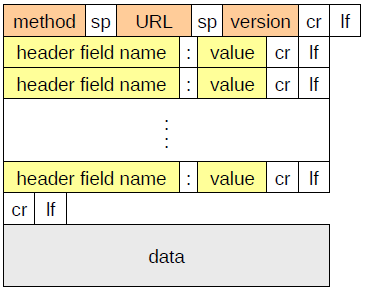
\includegraphics[width=0.5\textwidth]{img/HTTP_RequestHeader}
    \end{center}
    \item Trennung: Leerzeile
    \item Länge: Als Attribut im Header (content-length)
\end{itemize}

\minisec{Welche Gruppen von HTTP Status-Codes kennen Sie?}
\begin{itemize}
    \item 1xx – Informationen
    \item 2xx – Erfolgreiche Operation
    \item 3xx – Umleitung
    \item 4xx – Client-Fehler
    \item 5xx – Server-Fehler
    \item 9xx – Proprietäre Fehler
\end{itemize}

\minisec{Welche HTTP-Methoden existieren neben 'GET'?}
\begin{itemize}
    \item \textbf{HEAD}
    \item \textbf{POST}
    \item \textbf{PUT}
    \item \textbf{DELETE}
\end{itemize}

\minisec{Was ist MIME? Welche Attribute (mind. 3) im Header werden dazu verwendet, und was bedeuten (bzw. definieren) sie jeweils?}
\begin{itemize}
    \item \textbf{MIME} = \textbf{M}ultipurpose \textbf{I}nternet \textbf{M}ail \textbf{E}xtensions
    \item Attribute:
    \begin{itemize}
        \item \textcolor{blue}{Content-Type:} \textbf{IMAGE/JPEG}; name="picture.jpg"
        \item \textcolor{blue}{Content-Transfer-Encoding:} \textbf{BASE64}
        \item \textcolor{blue}{Content-ID:} <PINE.LNX.3.91.960212212235.325B@localhost>
    \end{itemize}
\end{itemize}

\minisec{Erklären Sie das Konzept von 'Virtual Hosts' bei HTTP!}
\begin{itemize}
    \item Auf einem Rechner sollen verschiedene Domains und Web-Server zur Verfügung stehen → Jeder Server hat die gleiche IP, aber ggf. unterschiedliche DNS-Namen!
    \item Ein oder mehrere Webserver (Software) sollen die Anfragen, für die auf dem Rechner vorhandenen Domains, beantworten
    \item Typische Anwendung: Web-Hosting (Provider)
\end{itemize}

\minisec{Wo ist der SSL-Layer im ISO/OSI oder Internet-Schichtenmodell angesiedelt?}
In der Darstellungsschicht (Schicht 6)

\minisec{Erklären Sie die Unterschiede/Vorteile/Nachteile von symmetrischer und asymmetrischer Verschlüsselung!}
\begin{itemize}
    \item Symmetrische Verschlüsselung:
    \begin{itemize}
        \item schneller
        \item braucht weniger Rechenleistung
        \item Schlüssel muss allerdings an jeden verteilt werden, der die Daten entschlüsseln muss
    \end{itemize}
    \item Asymmetrische Verschlüsselung:
    \begin{itemize}
        \item sicherer
        \item langsamer, da mehr Rechenleistung zum Entschlüsseln gebraucht wird
        \item Schlüssel müssen nicht an alle verteilt werden (private und public Key)
    \end{itemize}
\end{itemize}

\minisec{Was ist ein Zertifikat? Wer stellt es aus, und welche Informationen enthält es?}
Ein digitales Zertifikat ist ein digitaler Datensatz, der bestimmte Eigenschaften von Personen oder Objekten bestätigt und dessen Authentizität und Integrität durch kryptografische Verfahren geprüft werden kann.
Das digitale Zertifikat enthält insbesondere die zu seiner Prüfung erforderlichen Daten.
Die Ausstellung des Zertifikats erfolgt durch eine offizielle Zertifizierungsstelle, die Certification Authority (CA).

\minisec{Welche Eigenschaften hat eine Hash-Funktion? Wo wird Sie im Kontext der Verschlüsselung eingesetzt?}
\begin{itemize}
    \item \textcolor{blue}{Surjektivität} – Kein Ergebniswert (Hashwert) soll unmöglich sein, jedes Ergebnis (jeder Hashwert im definierten Wertebereich) soll tatsächlich vorkommen können.
    \item \textcolor{blue}{Effizienz} – Die Funktion muss schnell berechenbar sein, ohne großen Speicherverbrauch auskommen (der Speicherbedarf des Hashwertes soll deutlich kleiner sein als jener des Schlüssels / Eingabewertes) und sollte die Quelldaten (Eingabewerte) möglichst nur einmal lesen müssen.
    \item Hash-Funktion wird verwendet, um die private Keys zu verschlüsseln
\end{itemize}

\minisec{Wie kann man bei 2 Kommunikationspartnern ein 'Geheimnis' (z.B. einen Schlüssel zur symmetrischen Verschlüsselung) erzeugen, ohne dieses Geheimnis über das Netzwerk oder einen anderen Kanal auszutauschen?}
\medskip
\includegraphics[width=\textwidth]{img/Diffie-Hellman-Schlüsselaustausch}

\minisec{Welche Aufgaben hat das SSL Handshake Protokoll und das SSL Record Protokoll?}
\begin{itemize}
    \item SSL Handshake Protokoll:
    \begin{itemize}
        \item Den stärksten gemeinsam unterstützten Algorithmus ermitteln
        \item Authentifikation der Kommunikationspartner (Client optional)
        \item Ermitteln eines Session Keys zur symmetrischen Verschlüsselung (optional)
    \end{itemize}
    \item SSL Record Layer:
    \begin{itemize}
        \item Vollständig getrennt vom Handshake Protokoll
        \item Verschickt Daten symmetrisch mit dem im Handshake ausgehandelten Verschlüsselungsalgorithmen und Session Keys
        \item Bildet zu jedem Datenblock einen Message Digest zur Sicherung der Integrität
    \end{itemize}
\end{itemize}

\minisec{Warum sollte 'einfaches' FTP heute nicht mehr verwendet werden?}
Zu unsicher, Übertragung der Login-Daten als Klartext \ldots

\minisec{Warum gibt es in einem typischen Heimnetzwerk Probleme mit dem FTP 'Active' Mode?}
In Heimnetzen wird typischerweise NAT verwendet, und beim 'Active' Mode horcht der Client für die Datenverbindung auf einem zufälligen Port und teilt diesen dem Server über die Kontrollverbindung mit.
Diese Daten (IP in einem privaten Netz und Portnummer) sind aber für den NAT-Router nicht sichtbar (weil auf Anwendungsebene übertragen), und können daher vom NAT-Router nicht 'übersetzt' werden.

\minisec{Informieren Sie sich über die Entstehungsgeschichte und Funktionalität von SSL und SSH!}
\begin{itemize}
    \item \url{https://de.wikipedia.org/wiki/Secure_Shell}
    \item \url{https://de.wikipedia.org/wiki/Transport_Layer_Security}
    \item \url{https://www.kreitiv.de/ssl-tls-und-ssh-verschluesselungsprotokolle/}
\end{itemize}

\minisec{Wie funktionieren SFTP und TFTP?}
\begin{itemize}
    \item \underline{SFTP:} FTP über SSH Session
    \item \underline{TFTP:}
    \begin{itemize}
        \item sehr einfaches Protokoll für den File-Transfer
        \item die Kommunikation läuft über Port 69 und benutzt UDP, nicht TCP
        \item hat keine Authentifizierung
        \item benutzt immer 512-Byte-Blöcke
    \end{itemize}
\end{itemize}

\minisec{Welches Protokoll wird zum Versenden von Emails verwendet? Was passiert konkret bei Versenden, und wie ist das DNS beteiligt?}
\begin{itemize}
    \item Simple Mail Transfer Protokoll (SMTP)
    \item Email-Übertragung:
    \begin{enumerate}
        \item User Agent erstellt E-Mail
        \item Aufteilen der E-Mail in Header und Body
        \item Überprüfen und Zwischenspeichern der E-Mail vom Message Transfer Agent
        \item MTA sucht Mailserver des Empfängers im DNS
        \item Mail wird an Mailserver verschickt
        \item Mail wird vom Ziel-MTA überprüft
        \item Mail wird vom Empfänger Mailserver gespeichert
    \end{enumerate}
\end{itemize}

\minisec{Welche Protokolle werden zum Abrufen von Emails verwendet, und wie unterscheiden sie sich?}
\begin{itemize}
    \item \textcolor{blue}{Simple Mail Transfer Protocol (SMTP):}
    \begin{itemize}
        \item Versenden von E-Mails über TCP-Verbindung (Port 25)
        \item SMTP ist ein einfaches ASCII-Protokoll
        \item Ohne Prüfsummen, ohne Verschlüsselung
        \item Ist der Server zum Empfangen bereit, signalisiert er dies dem Client.
        Dieser sendet die Information, von wem die E-Mail kommt und wer der Empfänger ist.
        Ist der Empfänger dem Server bekannt, sendet der Client die Nachricht, der Server bestätigt den Empfang.
    \end{itemize}
    \item \textcolor{blue}{Post Office Protocol Version 3 (POP3):}
    \begin{itemize}
        \item Abholen der eMails beim Server über eine TCP-Verbindung, Port 110
        \item Befehle zum An- und Abmelden, Nachrichten herunterladen, Nachrichten auf dem Server löschen oder liegen lassen, Nachrichten ohne vorherige Übertragung vom Server direkt löschen
    \end{itemize}
    \item \textcolor{blue}{IMAP (Interactive Mail Access Protocol):}
    \begin{itemize}
        \item Hier werden die eMails nicht abgerufen und lokal gespeichert, sondern bleiben auf dem Server liegen!
    \end{itemize}
\end{itemize}

\minisec{Warum ist einfaches SMTP unsicher?}
\begin{itemize}
    \item Unverschlüsseltes, ASCII-basiertes Protokoll, Passwörter im Klartext.
    \item Einfache Möglichkeit zur Manipulation von E-Mails
\end{itemize}

\minisec{Wozu dient das (veraltete) TELNET-Protokoll? Wozu kann es (z.B. im Praktikum) sinnvoll eingesetzt werden?}
\begin{itemize}
    \item TCP ermöglicht den transparenten, interaktiven Gebrauch von „entfernten“ Maschinen
    \item verbreitetes Protokoll: TELNET, welches auf einer Client/Server-Kommunikation basiert
    \item Ein „Pseudo-Terminal“ des Servers interpretiert Zeichen, als kämen sie von der eigenen Tastatur
    \item bei Antwort des Servers umgekehrter Weg (Pseudo-Terminal fängt Antwort ab, leitet sie über TCP an den Client weiter, der die Ausgabe am Bildschirm macht
    \item \textbf{Benutzername und Passwort werden unverschlüsselt übertragen}
\end{itemize}

\minisec{Welches Protokoll sollte heute zum Login auf entfernten Rechnern verwendet werden?}
\begin{itemize}
    \item \textcolor{blue}{ssh} adressiert die Sicherheitsprobleme von telnet und rlogin.
    Es ist ein Protokoll zur Erstellung einer sicheren Verbindung zwischen zwei Systemen.
    Alle während der Verbindung gesendeten und empfangenen Daten werden mit einer 128 Bit-Verschlüsselung verschlüsselt.
    \item \textcolor{blue}{ssh} unterstützt verschiedene Authentisierungsarten:
    \begin{itemize}
        \item Bei der sogenannten hostbased-Authentifizierung akzeptiert ein Rechner ohne eigene account-spezifische Tests die Vorgaben eines fremden Rechners.
        Es wird höchstens die Identität des fremden Rechners überprüft.
        \item Die Authentifikation mit einem Passwort ist derzeit die "übliche" Methode, um sich an einem Rechner anzumelden.
        Die Sicherheit dieses Mechanismus beruht auf der Geheimhaltung des Passwortes, dessen Übertragung allerdings verschlüsselt wird
        \item Um auch das Übertragen eines verschlüsselten Passwortes zu vermeiden, werden die sogenannten public-key-Verfahren eingesetzt
    \end{itemize}
\end{itemize}

\minisec{Wie kann mein einen sicheren 'Tunnel' zu/von einem beliebigen (TCP-) Port einrichten?}
Mit \textcolor{blue}{SSH: Port-Forwarding:}
\begin{itemize}
    \item verschlüsselte Verbindung zwischen zwei beliebigen Ports
    \item kann auch ohne Shell genutzt werden
    \item lokaler Port führt direkt auf den Zielport, als wäre dieser lokal
\end{itemize}

\minisec{Wozu wird SNMP verwendet? Welches Transportprotokoll verwendet es? Was ist ein SNMP-Agent und eine MIB?}
\begin{itemize}
    \item Transportprotokoll: UDP
    \item SNMP: Protokoll, das festlegt, wie Management-Information kommuniziert wird (Formate und Bedeutung von SNMP-Nachrichten)
    \item MIB (Management Information Base): Die MIB spezifiziert die Informationseinheiten (items), die vorgehalten werden müssen, und welche Operationen darauf erlaubt sind.
    \item SNMP wird zum Management von Geräten im Netz verwendet (Fehlerstatus etc.)
\end{itemize}
    \addsec{Vorlesung 10 - Sicherungsschicht}

\minisec{In welche zwei Sublayer kann der Data-Link Layer (Schicht 2 in ISO/OSI) unterteilt werden? Was sind grob die Aufgaben dieser zwei Sublayer?}
\begin{itemize}
    \item LLC Sublayer: Das Protokoll LLC fügt einem gegebenen Datenpaket aus einer übergeordneten Schicht (meist der OSI-Schicht 3 „Vermittlungsschicht“) drei Felder hinzu:
    \begin{itemize}
        \item zwei jeweils 8 Bit bzw.\ 1 Byte große Kennzeichen:
        \begin{itemize}
            \item DSAP (Destination Service Access Point: Einsprungadresse des Empfängers)
            \item SSAP (Source Service Access Point: Einsprungadresse des Absenders)
        \end{itemize}
        \item ein 1 oder 2 Byte großes Feld Control mit Steuerinformationen für Hilfsfunktionen wie z. B. die Datenflusssteuerung
    \end{itemize}
    \item MAC Sublayer:
    \begin{itemize}
        \item Das \textbf{Kanalzugriffsprotokoll} beschreibt, nach welchen Regeln auf ein Übertragungsmedium zugegriffen werden darf,
        d.\ h. ein Rahmen auf der Verbindungsleitung übertragen werden darf
        \item Bei \underline{Punkt-zu-Punkt}-Verbindungen ist das Leitungszugriffsprotokoll einfach.
        \item Der Sender kann einen Rahmen senden, wann immer die Verbindungsleitung frei ist (bei vollduplex immer)
        \item Bei \underline{Multi-Access-Netzen} teilen sich mehrere Teilnehmer eine Verbindungsleitung, z. B. nach dem Bus-Prinzip.
        \item Hier übernimmt der MAC Layer die Koordination der Leitungsnutzung
        \item Der MAC-Layer liefert eine eindeutige Kennung für jedes Netzwerkgerät bzw.\ jede Netzwerk-Karte → \textcolor{blue}{MAC} Adresse
    \end{itemize}
\end{itemize}

\minisec{Welche Übertragungsmedien (auf Schicht 1 in ISO/OSI) werden heute typischerweise eingesetzt?}
\begin{itemize}
    \item Kupferdoppelader (Twisted Pair)
    \item Koaxialkabel
    \item Funk
    \item Glasfaser
\end{itemize}

\minisec{Welche physikalischen Größen werden dabei verwendet, und wie können diese moduliert werden?}
\begin{itemize}
    \item Spannung
    \item Elektromagnetische Wellen (Funk, Licht)
    \item Modellierung über:
    \begin{itemize}
        \item Amplitude
        \item Frequenz
        \item Phase
    \end{itemize}
    \item Die Veränderung dieser Eigenschaften im Rahmen
    der Datenübertragung nennt man \textcolor{blue}{Modulation}
    \begin{itemize}
        \item Amplitudenmodulation (AM)
        \item Frequenzmodulation (FM)
        \item Phasenmodulation (PM)
    \end{itemize}
\end{itemize}

\minisec{Welche unterschiedlichen Arten von 'twisted pair'-Kabeln kennen Sie?}
\begin{itemize}
    \item Unterscheidung nach Kategorie:
    \begin{itemize}
        \item \textcolor{blue}{Kategorie 3 :} Gemeinsame Umhüllung für vier Kupferdoppeladern
        \item \textcolor{blue}{Kategorie 5 :}
        Wie Kategorie 3, aber mehr Windungen/cm (weitere Reduktion der elektromagnetischen Interferenzen Umhüllung besteht aus Teflon (bessere Isolierung, Qualität der Signale bleibt auf längere Strecken akzeptabel)
        \item \textcolor{blue}{Kategorie 6,7 :} Die Paare sind zusätzlich einzeln mit Silberfolie umwickelt
    \end{itemize}
    \item Unterscheidung nach Abschirmung:
    \begin{itemize}
        \item \textcolor{blue}{UTP Kabel (Unshielded Twisted Pair) :} Keine Abschirmung des Kabels
        \textcolor{blue}{STP Kabel (Shielded Twisted Pair) :} Abschirmung des Kabels, dadurch günstigere Eigenschaften, trotzdem in der Praxis oft UTP
    \end{itemize}
    \item Beispiele: S/UTP-Kabel (cat 5), S/STP-Kabel (cat 7)
\end{itemize}

\minisec{Wie ist ein Glasfaserkabel prinzipiell aufgebaut? Wo findet die 'Übertragung' statt?}
\begin{itemize}
    \item Von innen nach außen:
    \begin{enumerate}
        \item Faserkern / Kernglas (core)
        \item Mantelglas (cladding)
        \item Beschichtung (coating)
        \item Kunststoffummantelung (buffering)
        \item Schutzmantel
    \end{enumerate}
    \item Im Glaskern findet die Übertragung statt
\end{itemize}

\minisec{Erklären Sie im Zusammenhang mit Glasfaserkabeln die Begriffe 'Moden' und 'Dispersion'!}
\begin{itemize}
    \item Dispersion
    \begin{itemize}
        \item Begrenzt Übertragungsstrecke
        \item Lichtpuls besteht aus mehreren Wellen (Strahlen) → Einfallswinkel dieser Strahlen unterschiedlich
        \item Lichtstrahlen kommen im Medium unterschiedlich schnell vorwärts:
        \begin{itemize}
            \item Wege (\textbf{Moden}) der Strahlen unterschiedlich lang (abhg.\ von Einfallswinkel)
            \item Strahlen eines Impulses kommen zeitversetzt am Ende des Kabels an
            \item Intensität der Impulse nimmt ab, benachbarte Impulse verschwimmen
        \end{itemize}
        \item (Weitere Faktoren können ebenso Dispersion verursachen)
    \end{itemize}
\end{itemize}

\minisec{Wie unterscheiden sich Monomode- und Multimode Glasfaserkabel? Welche Eigenschaften resultieren aus dem unterschiedlichen Aufbau?}
\begin{itemize}
    \item Monomode-Faser
    \begin{itemize}
        \item Kerndurchmesser: 8--10 $\mu m$
        \item Alle Strahlen können nur noch einen Weg nehmen
        \item Keine Dispersion (homogene Signalverzögerung)
        \item 50 $\frac{GBit}{s}$ über 100 km
        \item Teuer wegen geringem Kerndurchmesser
    \end{itemize}
    \item Multimode-Faser mit Stufenindex
    \begin{itemize}
        \item Kerndurchmesser: 50 $\mu m$
        \item Unterschiedliche Wege für Lichtwellen, je nach Einfallswinkel
        \item Starke Dispersion
        \item Bis zu 1 km
    \end{itemize}
    \item Multimode-Faser mit Gradientenindex
    \begin{itemize}
        \item Kerndurchmesser: 50 $\mu m$
        \item Brechungsindex ändert sich fließend
        \item Leicht unterschiedliche Wege für Lichtwellen
        \item Geringe Dispersion
        \item Bis zu 30 km
    \end{itemize}
\end{itemize}

\minisec{Bei welcher Netztopologie gibt es ein 'gemeinsames' Medium, auf das alle Teilnehmer zugreifen?}
Multi-Access-Netz (gemeinsames Medium)
\begin{itemize}
    \item Nur in lokalen Netzen verwendet
    \item Alle Stationen sind an ein einziges Medium angeschlossen
    \item Sendet eine Station Daten, werden sie an alle Stationen ausgeliefert
    \item Jeder Rechner kontrolliert jedes Paket, ob es für ihn bestimmt ist
\end{itemize}

\minisec{Bei welchen Netztopologien gibt es ausschließlich Punkt-zu-Punkt-Verbindungen zwischen den Teilnehmern?}
\begin{itemize}
    \item Stern
    \item Ring
    \item Baum (mit Stern Verbindungen)
\end{itemize}

\minisec{Vergleichen Sie Ring-, Bus- und Stern-Topologie bzgl. ihrer Vor- und Nachteile!}
\begin{itemize}
    \item Ring: Point-to-Point
    \begin{itemize}
        \item Reihe von Punkt-zu-Punkt-Verbindungen
        \item Aktive Knoten: fungieren als Repeater
        \item Ausfall des gesamten Rings bei Unterbrechung einer Verbindung
        \item Ausfall des gesamten Rings bei Ausfall eines Knotens (Bypass als Abhilfe)
        \item Große Ausdehnung möglich (aufgrund der aktiven Knoten)
        \item Einfaches Einfügen neuer Knoten
        \item Variante: bidirektionaler Ring: Knoten sind durch zwei gegenläufige Ringe miteinander verbunden
    \end{itemize}
    \item Bus: Multi-Access-Netz
    \begin{itemize}
        \item + Einfach, preiswert, einfacher Anschluss neuer Knoten
        \item + Passive Ankopplung der Stationen, der Ausfall eines Knotens ist kein Problem für die anderen Knoten
        \item – Nur eine Station zu einem Zeitpunkt kann senden;
        alle anderen Stationen können nur empfangen
        \item – Begrenzung der Zahl anschließbarer Stationen
        \item – Passive Ankopplung der Stationen, daher begrenzte Ausdehnung des Busses (aber: Repeater zur Kopplung mehrerer Busse)
    \end{itemize}
    \item Stern
    \begin{itemize}
        \item Ausgezeichneter Knoten als zentrale Station
        \begin{itemize}
            \item Nachricht von Station A wird durch die zentrale Station an Station B weitergeleitet
            \item Punkt-zu-Punkt-Verbindungen (\textcolor{blue}{Switch}), oder Broadcast (\textcolor{blue}{Hub})
            \item Verwundbarkeit durch zentralen
        \end{itemize}
        \item Knoten (Redundanz möglich)
    \end{itemize}
\end{itemize}

\minisec{Wie (und auf welcher Schicht) arbeitet ein Repeater?}
\begin{itemize}
    \item Verknüpfung von zwei Netzen zur Vergrößerung der Ausdehnung
    \item Arbeitet auf der Bitebene
    \begin{itemize}
        \item Kann einkommende Signale als „0“ oder „1“ interpretieren
        \item Empfang und \textcolor{blue}{Auffrischung} des Signals – ein empfangenes Bit wird auf der anderen Seite neu als Stromimpuls codiert
        \item Kein Verstehen von Adressen höherer Schichten, alle Daten werden weitergeleitet (das Netz bleibt z.\ B. ein Multi-Access-Netz)
    \end{itemize}
\end{itemize}

\minisec{Erklären Sie (im Kontext eines Netzes mit twisted-pair Kabeln) den Unterschied zwischen einem Hub und einem Switch!}
\begin{itemize}
    \item Hub = „Repeater mit mehr als zwei Anschlüssen“
    \begin{itemize}
        \item Signalauffrischung wie beim Repeater
        \item An einen Anschluss kann ein einzelner Rechner oder ein ganzer Bus angeschlossen werden
        \item Multi-Access-Netz: der Hub gibt ein empfangenes Signal auf allen Anschlüssen wieder aus, praktisch wie ein "Bus" mit mehreren Anschlüssen:
        \item \textcolor{blue}{Gemeinsamer Übertragungskanal}, d.\ h. Stationen können nicht gleichzeitig senden und empfangen, nur eine Station auf einmal kann senden
        \item Geringe Sicherheit, da alle Stationen mithören können
    \end{itemize}
    \item Switch - Wie Hub, aber:
    \begin{itemize}
        \item Punkt-zu-Punkt-Kommunikation zwischen zwei Stationen
        \begin{itemize}
            \item Switch kann Layer-2-Adressen (MAC-Adressen) der angeschlossenen Stationen verstehen, lernt sie und kann Daten gezielt weiterleiten
            \item Stationen können gleichzeitig senden und empfangen
            \item Nur der adressierte Empfänger erhält die Daten, andere Stationen können nicht mithören
        \end{itemize}
        \item Vermeidung von Kollisionen (‚Mikrosegmentierung‘)
        \item Puffer für jeden Port
    \end{itemize}
\end{itemize}

\minisec{Was ist ein 'Layer-3 Switch'?}
\begin{itemize}
    \item Ein Layer-3-Switch ist eine Kombination aus Router und Switch.
    \item Er beherrscht nicht nur Switching, sondern auch Routing.
    \item Da Router und Switche sehr ähnlich funktionieren – sie empfangen, speichern und leiten Datenpakete weiter – ist es nur logisch beide Geräte miteinander zu kombinieren, um daraus ein Multifunktionsgerät zu machen.
\end{itemize}

\minisec{Warum gibt es in der Schicht 2 neben dem Header auch einen Trailer? Welche Felder enthält der Ethernet-Header?}
\begin{itemize}
    \item Trailer:
    \begin{itemize}
        \item Frame Check Sequence (CRC Prüfsumme)
    \end{itemize}
    \item Header:
    \begin{itemize}
        \item MAC Empfänger
        \item Absender
        \item Ethernet Typ
    \end{itemize}
\end{itemize}
    \addsec{Vorlesung 11 - Kanalzuteilung, Fehlerkorrektur}

\minisec{Welche Aufgabe hat der MAC Sublayer in der Schicht 2 (Wiederholungsfrage, siehe Vorlesung 10)?}
\begin{itemize}
    \item \todo A
\end{itemize}

\minisec{Welche Eigenschaften hätte ein ideales Mehrfachzugriffsprotokoll?}
Broadcast-Medium mit Maximalrate R bps
\begin{itemize}
    \item Ein einzelner Knoten kann mit der Rate R übertragen
    \item M Knoten können mit einer mittleren Rate von $\frac{R}{M}$ übertragen
    \item Das Protokoll ist dezentral, d.h. es gibt keine Master-Knoten, die ausfallen und das ganze System zum Absturz bringen können
    \item Das Protokoll ist einfach und kann somit kostengünstig implementiert werden
\end{itemize}

\minisec{Nennen Sie 3 grundsätzliche Strategien, wie der mehrfache Zugriff auf ein gemeinsames Medium gelöst werden kann!}
\begin{itemize}
    \item \textcolor{blue}{Kanalaufteilungsprotokolle (Multiplexing)}
    \begin{itemize}
        \item Aufteilung des Übertragungskanals in kleine Übertragungseinheiten (Zeitfenster, Frequenzen, Kodierung)
        \item Exklusive Nutzung der Übertragungseinheiten für einzelne Knoten
    \end{itemize}
    \item \textcolor{blue}{Zufallszugriffsprotokolle}
    \begin{itemize}
        \item Keine Unterteilung des Kanals, jeder überträgt mit der gesamten Leitungskapazität.
        Allerdings sind \underline{Kollisionen} von Nachrichten möglich und müssen korrekt behandelt werden
    \end{itemize}
    \item \textcolor{blue}{Rotationsprotokolle}
    \begin{itemize}
        \item Der Zeitpunkt, wann ein Knoten senden kann wird durch eine spezielle Koordinierung nach einem flexiblen Rotationsprinzip im Übertragungsmedium ausgetauscht.
    \end{itemize}
\end{itemize}

\minisec{Erklären Sie kurz die Funktionsweise von TDMA, FDMA und CDMA!}
\begin{itemize}
    \item \textcolor{blue}{TDMA: Time Division Multiple Access:}
    \begin{itemize}
        \item Aufteilung des Kanals in kleine Zeiteinheiten, die sich in Runden wiederholen
        \item Jeder Knoten kann eine bestimmte Anzahl an Zeiteinheiten in jeder Runde Nutzen
        \item Ungenutzte Einheiten (slots) bleiben ungenutzt
        \item Die Zeiteinheiten können meist auch gruppiert angefordert werden
        \item Anforderung entspricht Konfiguration der NIC-Karte
    \end{itemize}
    \item \textcolor{blue}{FDMA: Frequency Division Multiple Access}
    \begin{itemize}
        \item Aufteilung des Kanals in Frequenzbänder
        \item Nach Nyquist kann ein rauschfreier Kanal mit einem Frequenzband der Breite x Hz binäre Signale nicht mit mehr als 2x Bps übertragen (Nyquist-Bandbreite)
        \item Jede Station nutzt ein Frequenzband
        \item Die Kapazität nicht genutzter Frequenzbänder geht verloren
    \end{itemize}
    \item \textcolor{blue}{CDMA: Code Division Multiple Access}
    \begin{itemize}
        \item Keine Unterteilung in Zeitslots oder Frequenzen
        \item Nutzung von ‚orthogonalen Codes‘ bei der (De-) Modulation, die sich im Medium überlagern/mischen, aber trotzdem auf Empfängerseite eindeutig wiederhergestellt werden können
        \item Vorteil: Es gibt keine ungenutzten Resourcen wie bei TDMA/FDMA
    \end{itemize}
\end{itemize}

\minisec{Erklären Sie die Funktionsweise von CSMA/CD! Was bedeutet diese Abkürzung?}
\begin{itemize}
    \item \textcolor{blue}{Carrier Sense Multiple Access (CSMA)}
    \begin{itemize}
        \item höre vor der Übertragung das Medium ab
        \item sende nur, falls das Medium frei ist
        \item Analogie: Unterbreche keine Anderen
    \end{itemize}
    \item \textcolor{blue}{Carrier Sense Multiple Access with Collision Detection (CSMA/CD)}
    \begin{itemize}
        \item wie CSMA, zusätzlich: höre während der Sendung das Medium weiter ab und breche die Übertragung ab, wenn eine Kollision auftritt
        \item sende ein Jamming-Signal, damit jede Station weiß, dass eine Kollision aufgetreten ist und die Nachricht nutzlos geworden ist.
        \item Wichtig: Man muss so lange senden, dass man ein Jamming -Signal während dessen auch mitbekommt
    \end{itemize}
\end{itemize}

\minisec{Erklären Sie, warum bei CSMA/CD ein Sender eine Mindestzeit senden muss (und parallel per "CD" das Medium abhören muss)! Wie lässt sich diese Mindestzeit berechnen und ggf. in eine Mindest-Rahmengröße umrechnen?}
\begin{itemize}
    \item
\end{itemize}

\minisec{Wie funktioniert und wozu dient der "Binary Exponential Backoff"-Algorithmus?}
Um nach einer Kollision die gleichzeitige Wiederholung der kollidierten Sendungen
zu vermeiden (Folgekollision), wird eine zufällige Wartezeit aus einem vorgegebenen
Intervall gezogen.
Das Intervall wird \textit{klein} gehalten, um große Wartezeiten
bis zur Wiederholung zu vermeiden.
Dadurch ist allerdings das Risiko eines
Folgekonflikts groß.
Kommt es so zu einer weiteren Kollision, wird das Intervall
vor dem nächsten Versuch vergrößert, um mehr Spielraum für alle sendenden
Parteien zu schaffen.

\minisec{Welche heute typischerweise eingesetzten Ethernet-Standards kennen Sie? Wie sind die Namen aufgebaut?}
Basiert auf IEEE 802.3 „CSMA/CD“
4 Klassen von Ethernet-Varianten:
\begin{itemize}
    \item Standard Ethernet → 10 $\frac{Mb}{s}$
    \item Fast Ethernet → 100 $\frac{Mb}{s}$
    \item Gigabit Ethernet → 1000 $\frac{Mb}{s}$
    \item 10Gigabit-Ethernet → 10000 $\frac{Mb}{s}$
\end{itemize}

\minisec{Warum wurde bei Gigabit-Ethernet die minimale Rahmenlänge von 64 auf 520 Bytes erhöht?}
\begin{itemize}
    \item  \todo A
\end{itemize}

\minisec{Warum wurde bei Fast-Ethernet die Segmentlänge von 2500m (10MBit Ethernet) auf 200--250m verkleinert?}
Die minimale Rahmenlänge zur Kollisionserkennung bei Ethernet beträgt 64 Byte.
Bei 100 Mb/s wird der Rahmen aber ca. 10 Mal so schnell abgesendet, so dass eine Kollisionserkennung nicht mehr gewährleistet ist.

\minisec{Wie ist die Rahmen-Struktur eines Ethernet-Paketes aufgebaut? Welche Daten (-Felder) werden im Header und Trailer auf Schicht 2 übertragen?}
Ethernet-Rahmen:
\begin{itemize}
    \item \textcolor{blue}{\textit{Präambel :}} kennzeichnet eine folgende Übertragung und synchronisiert den Empfänger mit dem Sender.
    \item Der \textcolor{blue}{\textit{Start-of-Frame-Delimiter :}} (bzw. die beiden aufeinanderfolgenden Einsen) zeigen an, dass endlich Daten folgen.
    \item \textcolor{blue}{\textit{Destination Address :}} das erste Bit kennzeichnet den Empfänger: entweder eine einzelne Station (1. Bit = 0) oder eine Gruppenadresse (1. Bit = 1; Broadcast ist auch hier durch 11 \ldots 1 gegeben).
    \item \textcolor{blue}{\textit{Length/Type :}} Bei einem Wert bis 1500 wird die Angabe als Länge des Datenteils aufgefasst (dies ist der Fall beim so genannten CSMA/CD), bei einem Wert ab 1536 wird hier angegeben, an welches Schicht-3- Protokoll die Daten weitergegeben werden sollen (verwendet bei Ethernet).
    \item \textcolor{blue}{\textit{FCS :}} Checksumme, 32-Bit CRC. Diese erstreckt sich über die Felder DA, SA, Length/Type, Data/Padding.
\end{itemize}
Felder in Schicht 2:
\begin{itemize}
    \item MAC-Empfänger
    \item MAC-Absender
    \item 802.1Q-Tag (opt.)
    \item EtherType
    \item Nutzlast (1500 bytes)
    \item Frame Check Sequence
\end{itemize}

\minisec{Erklären Sie die grundsätzliche Vorgehensweise des Medienzugriffes beim Token-Ring Netz!}
\begin{itemize}
    \item “Token“-Verfahren, nur wer ein bestimmtes Token ( = Bitfolge) besitzt, darf senden
    \item Die Rechner teilen sich einen Ring aus Punkt-zu-Punkt- Verbindungen
    \item Das Token wird zyklisch weitergegeben
\end{itemize}

\minisec{Was ist ein Hamming-Abstand bei einem Code C mit den Wörtern $c_1$ bis $c_n$?}
\begin{itemize}
    \item Anzahl unterschiedlicher Bits zweier Codewörter $c_1$ und $c_2$, d. h. Anzahl der 1-Bits von $c_1$ XOR $c_2$.
    \item Beispiel: d(10001001, 10110001) = 3
    \item Hamming-Abstand D von vollständigem Code C : \[ D(c)\coloneqq \min\{d(c_1 ,c_2)\ |\ c_1 ,c_2\ \epsilon \ C; \ c_1 \neq c_2\}\]
\end{itemize}

\minisec{Was versteht man unter "Forward Error Correction"?}
\begin{itemize}
    \item \todo A
\end{itemize}

\minisec{Wie groß muss der Hamming-Abstand mindestens sein, um e-Bitfehler zu erkennen bzw. zu beheben?}
\begin{itemize}
    \item \textcolor{blue}{erkennen} von e-Bit-Fehlern: Hamming-Abstand \textcolor{blue}{e+1} notwendig
    \item \textcolor{blue}{beheben} von e-Bit-Fehlern: Hamming-Abstand \textcolor{blue}{2e+1} notwendig
\end{itemize}

\minisec{Nennen Sie einen Code, der mit einer minimalen Anzahl von Prüfbits Einzelbitfehler korrigieren kann!}
\begin{itemize}
    \item \todo A
\end{itemize}

\minisec{Was versteht man unter Modulo-2 Arithmetik? Wie werden Addition und Subtraktion durchgeführt?}
\begin{itemize}
    \item Die Rechenoperationen werden in der Modulo-2-Arithmetik einfacher, da hierbei keine Überträge zu berücksichtigen sind!
    \item Addition und Subtraktion führen so zu dem gleichen Ergebnis.
    \item Wir können einfach mit XOR arbeiten!
    \item Digitaltechnik, hier Halbaddierer: Eine Addition ist logisch ein XOR, das Carry ein UND
    \item Es gibt eine Bitkombination n, sodass gilt: $(D \cdot 2^r) XOR \ R = n G$
    \item D.h., R soll so gewählt werden, dass G in $D \cdot 2^r$ ohne Rest teilbar ist
    \item $D \cdot 2^r = nG \ XOR \ R$
    \item Damit kann man R berechnen, denn wenn man $D \cdot 2^r$ durch G teilt, ist der Rest des Wertes genau R
    \[R = Rest\left[\frac{D \cdot 2^r}{G}\right]\]
\end{itemize}

\minisec{Was leistet bzw. wie funktioniert das CRC-Verfahren? Wozu dient das Generator-Polynom?
Wo wird das Verfahren im Kontext von Ethernet eingesetzt?}
\begin{itemize}
    \item Polynom-Codes: Interpretiere Datenbits D als Bitkette eines Polynoms, dessen Koeffizienten die 0-1-Werte der Bitkette sind
    \item Prüfung basiert auf Polynom-Arithmetik
    \item Sender und Empfänger einigen sich auf ein gemeinsam verwendetes Bitmuster der Länge r+1 Bit, das als Generator G bezeichnet wird. Das höchstwertige Bit hiervon ist 1
    \item Konzept: Berechne die r CRC-bits R so, dass die d + r Bits (als Binärzahl interpretiert) mit der Modulo-2-Arithmetik genau durch G teilbar sind
    \begin{itemize}
        \item Empfänger kennt G, teilt <D,R> durch G. Falls der Rest ungleich 0, so liegt ein Fehler vor!
        \item Kann Burst-Fehler von weniger als r+1 Bits und jede ungerade Fehlerzahl erkennen
    \end{itemize}
\end{itemize}

    \addsec{Vorlesung 11 - Beispielaufgaben}

\minisec{Übungsaufgabe 1:}
Zur Berechnung einer CRC Prüfsumme soll das Generatorpolynom $x^5 + x^3 + x^2 + 1$ verwendet werden.
Berechnen Sie die CRC-Prüfsumme zur Bitfolge \textbf{11110111} und geben Sie an, welche Daten tatsächich gesendet werden!
    \addsec{Vorlesung 11 - Lösungen}

\minisec{Übungsaufgabe 1:}
Zur Berechnung der CRC Prüfsumme wird das Generatorpolynom in eine Bitfolge mit führender '1' umgewandelt:
\[1x^5 + 0x^4 + 1x^3 + 1x^2 + 0x^1 + 1x^0 ->  101101\]
Das Polynom ist also vom Grad 5, und wir müssen 5 Nullen an die zu sendenden Daten anhängen!
Danach rechnen wir so lange in Modulo-2 Arithmetik (XOR-Verknüpfungen), bis keine Bits mehr übrig sind:

\begin{center}
    \begin{tabular}{c c c c c c c c c c c c c}
        1 & 1 & 1 & 1 & 0 & 1 & 1 & 1 & 0 & 0 & 0 & 0 & 0 \tabularnewline
        1 & 0 & 1 & 1 & 0 & 1 & & & & & & & \tabularnewline
        \hline
        0 & 1 & 0 & 0 & 0 & 0 & 1 & & & & & & \tabularnewline
        & 1 & 0 & 1 & 1 & 0 & 1 & & & & & & \tabularnewline
        \hline
        & 0 & 0 & 1 & 1 & 0 & 0 & 1 & 0 & & & & \tabularnewline
        & & & 1 & 0 & 1 & 1 & 0 & 1 & & & & \tabularnewline
        \hline
        & & & 0 & 1 & 1 & 1 & 1 & 1 & 0 & & & \tabularnewline
        & & & & 1 & 0 & 1 & 1 & 0 & 1 & & & \tabularnewline
        \hline
        & & & & 0 & 1 & 0 & 0 & 1 & 1 & 0 & & \tabularnewline
        & & & & & 1 & 0 & 1 & 1 & 0 & 1 & & \tabularnewline
        \hline
        & & & & & 0 & 0 & 1 & 0 & 1 & 1 & 0 & 0 \tabularnewline
        & & & & & & & 1 & 0 & 1 & 1 & 0 & 1 \tabularnewline
        \hline
        & & & & & & & 0 & \textcolor{blue}{0} & \textcolor{blue}{0} & \textcolor{blue}{0} & \textcolor{blue}{0} & \textcolor{blue}{1} \tabularnewline
    \end{tabular}
\end{center}

Das Ergebnis der Prüfsummenberechnung ist 00001, d.\ h. die zu sendende Bitfolge ist: 11110111\textcolor{blue}{00001}
    \addsec{Vorlesung 12 - Leitungscodes, WLAN}

\minisec{Erklären Sie den Begriff Signalbildung (bzw. Leitungskodierung)!}
Signalbildung ist die Umwandlung der binären Sendedaten (nach eventueller Kompression und/oder Kodierung mit Prüfsummen etc.) in physikalische Signale.
Die Signale müssen dabei nicht unbedingt binär sein, sondern können auch mehr als 2 Zustände annehmen.

\minisec{Welche Anforderungen kennen Sie, die ein guter Leitungscode erfüllen sollte?}
\begin{itemize}
    \item Möglichst hohe \textcolor{blue}{Widerstandsfähigkeit gegen Dämpfung}
    \item \textcolor{blue}{Effizienz:} möglichst hohe Übertragungsraten durch Codewörter
    \begin{itemize}
        \item binärer Code: +5V / -5V?
        \item ternärer Code: +5 V / 0V / -5V?
        \item quaternärer Code: 4 Zustände (Codierung von 2 Bit gleichzeitig)
    \end{itemize}
    \item \textcolor{blue}{Taktrückgewinnung} beim Empfänger (\textcolor{blue}{Synchronisation}), dazu möglichst
    häufige/regelmäßige Pegelwechsel
    \item Gleichstromfreiheit: positive und negative Signale treten ungefähr gleich oft auf → kein nennenswerter elektrischer Gleichstrom-Fluss
    \item Robustheit: Können längere Sequenzen von 0 und 1 noch als solche noch erkannt werden?
    Können fehlerhafte Bits erkannt werden?
\end{itemize}

\minisec{Welche Vor- und Nachteile hat ein binärer gegenüber einem quaternären Code?}
\begin{itemize}
    \item Vorteil: Ein quaternärer Code kann 2 Nutzdatenbits in einem Code-Symbol abbilden
    \item Nachteil: Die Unterscheidung von 4 verschiedenen Signalzuständen kann anfälliger gegenüber Störungen bei der Übertragung sein.
\end{itemize}

\minisec{Erklären Sie den Unterschied zwischen Basisband- und Breitband-Übertragung!}
\begin{itemize}
    \item \textcolor{blue}{Basisband:} Das Basisband ist der natürliche Frequenzbereich des Nutzsignals (untere Grenzfrequenz $f_{\min}$ gleich oder nahe bei 0 Hz).
    Die digitalen Informationen werden ‚direkt‘ in physikalische Größen übersetzt und so über die Leitung übertragen.
    Hierzu sind Kodierungsverfahren notwendig, die festlegen, wie bei der Übertragung eine 0 bzw.\ eine 1 repräsentiert werden.
    Es kann nur je ein Signal übertragen werden
    \item \textcolor{blue}{Breitband:} Die digitalen Nutzdaten werden nicht direkt übertragen, sondern einem oder mehreren hochfrequenten Trägern aufmoduliert.
    Durch die Verwendung verschiedener Trägerwellen (Frequenzen) können dann mehrere Informationen gleichzeitig übermittelt werden
\end{itemize}

\minisec{Erklären Sie den Unterschied zwischen Bit- und Baudrate!}
\begin{itemize}
    \item Wenn die Zeitdauer (Schrittdauer) eines \textcolor{blue}{Symbols} bzw.\ \textcolor{blue}{Codeelements} $T$ ist,
    ist die Schrittgeschwindigkeit \[v_s = \frac{1}{T}\] (Einheit: \textcolor{blue}{Baud}), Symbolrate
    \item Die Übertragungsgeschwindigkeit (äquivalente Bitrate) ist dann \[v_u = v_s ld n\] ($n=$ Anzahl diskreter Zustände des Codeelements)
\end{itemize}
Bei binären Codeelementen stimmen somit \textcolor{blue}{Bitrate} und \textcolor{blue}{Baudrate} (Schrittgeschwindigkeit) überein, falls nur Codeelemente für Daten übermittelt werden (es gibt auch Codeelemente für z.\ B. die Rahmenstruktur)

\minisec{Was ist der Unterschied zwischen einem NRZ- und einem RZ-Code?}
\begin{itemize}
    \item \textbf{NRZ / NRZ-L: Non-Return\_to\_Zero:}
    \begin{itemize}
        \item Kein automatisches Zurückfallen auf einen Grundpegel.
        Hier z.\ B.:
        \item 0 = negative Spannung (konstant 0V), Pegel 1
        \item 1 = positive Spannung (konstant +5V), Pegel 2
        \item \underline{Nachteil:} bei langen 0 oder 1 Folgen \underline{Taktverlust} und \underline{keine Gleichstromfreiheit}
        \item \underline{Beispiel:} UART, RS232 (serielle Schnittstellen)
    \end{itemize}
    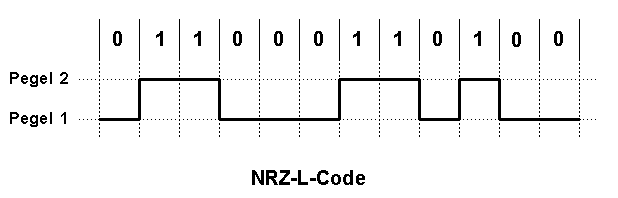
\includegraphics[width=0.8\textwidth]{img/NRZ-L-Code}
    \item \textbf{RZ: Return to Zero (hier unipolar)}
    \begin{itemize}
        \item 0 = 0V
        \item 1 = $\frac{T}{2}$ lang 1, $\frac{T}{2}$ lang 0
        \item \underline{Vorteil:} Taktrückgewinnung bei 1-Folgen
        \item \underline{Nachteil:} Keine Gleichstromfreiheit, kein Takt bei langen 0-Folgen
        \item \underline{Beispiel:} IrDA – Fernbedienung
    \end{itemize}
    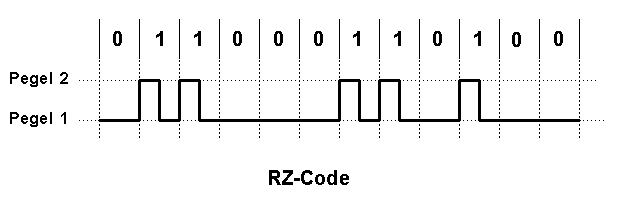
\includegraphics[width=0.8\textwidth]{img/RZ-Code}
\end{itemize}

\minisec{Welche Eigenschaften besitzt der Manchester-Code? Was bedeutet 1B2B?
Wie unterscheiden sich die Standards nach G.E. Thomas und IEEE 802.3?}
\begin{itemize}
    \item Eigenschaften:
    \begin{itemize}
        \item Lange Folgen gleicher Signale werden durch einen Pegelwechsel in
        der Mitte jedes Bits verhindert.
        Nach G.\ E. Thomas:
        \item 0 = Polaritätswechsel von negativ (-5V) nach positiv (+5V)
        \item 1 = Polaritätswechsel von positiv (+5V) nach negativ (-5V)
        \item \underline{Vorteil:} Gleichstromfrei, Taktrückgewinnung möglich
        \item \underline{Nachteil:} Doppelte Bandbreite im Vergleich zu NRZ, Bitrate $= \frac{Baudrate}{2}$
        \item \underline{Beispiel:} 10Base2
    \end{itemize}
    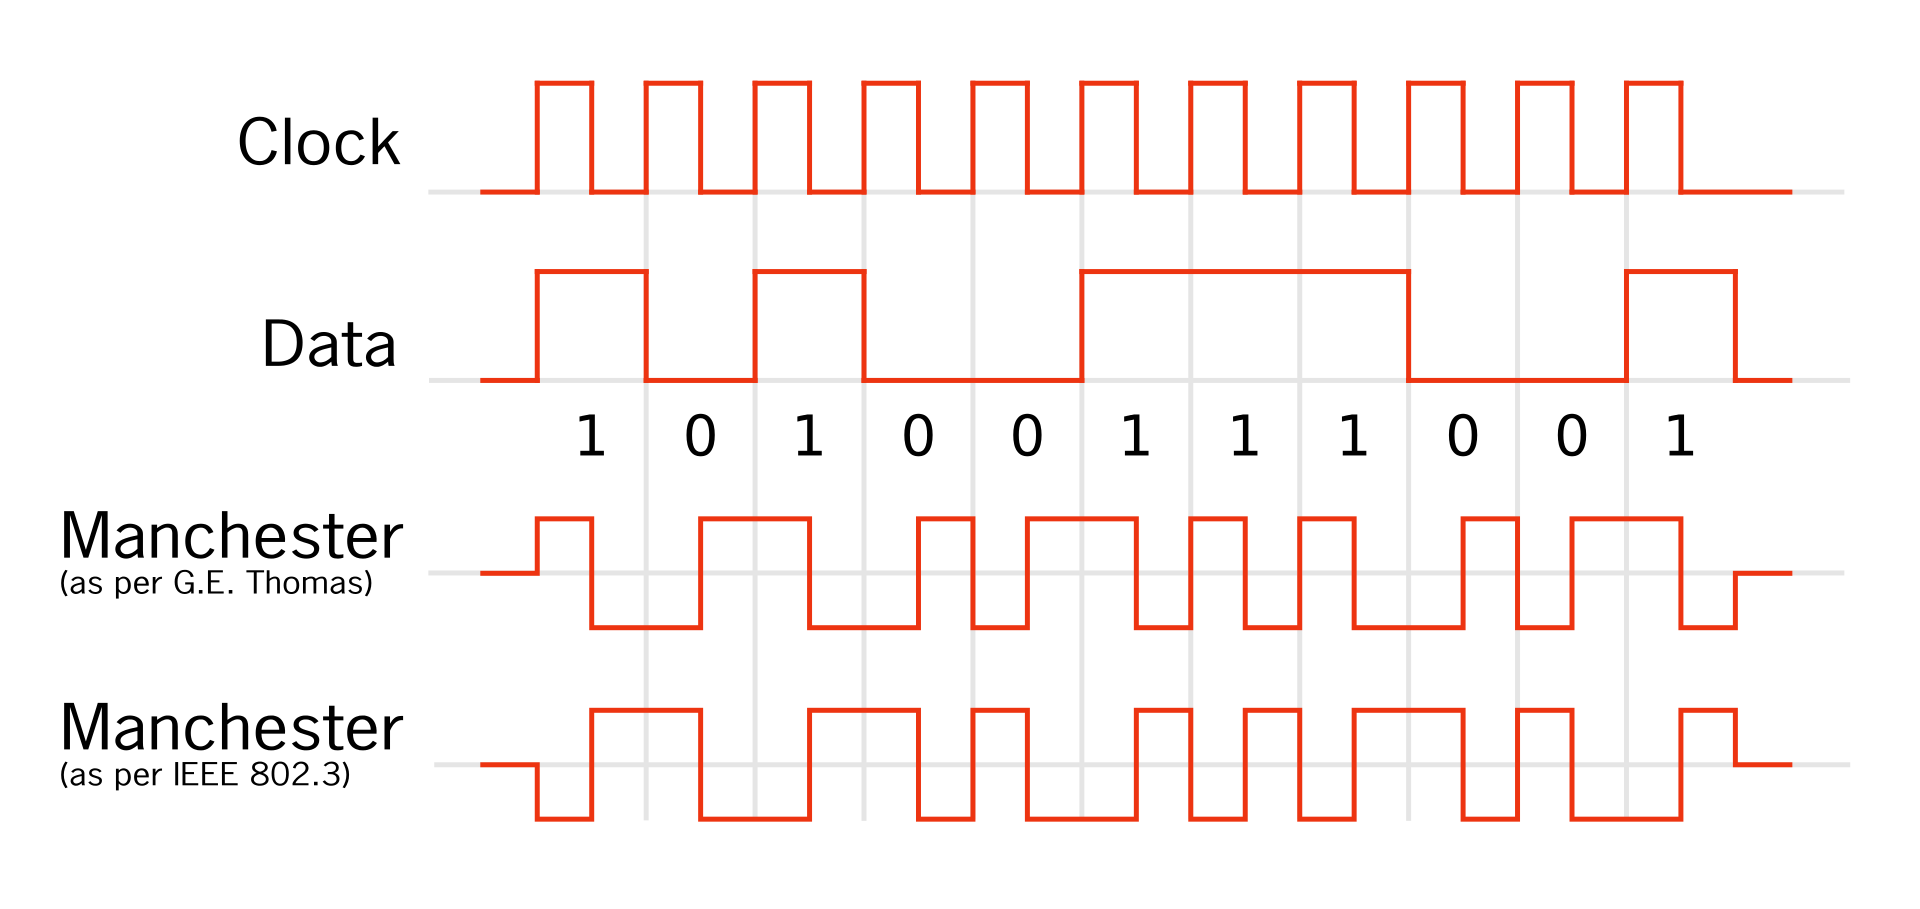
\includegraphics[width=\textwidth]{img/Manchester-Code}
    \item \textcolor{blue}{1B/2B-:} ein Bit wird auf zwei Symbole kodiert
\end{itemize}

\minisec{Welche Vorteile hat ein 4B/5B Code gegenüber einem 1B/2B Code?}
\begin{itemize}
    \item \underline{Nachteil des Manchester-Codes:}
    \begin{itemize}
        \item 50\% Effizienz, d.\ h. \textcolor{blue}{1B/2B-Code} (ein Bit wird auf zwei Symbole kodiert)
        Eine Verbesserung stellt der \textcolor{blue}{4B/5B-Code} dar:
        \item vier Bit werden in fünf Symbole kodiert: 80\% Effizienz
    \end{itemize}
    \item \underline{Arbeitsweise:}
    \begin{itemize}
        \item Pegelwechsel bei 1, kein Pegelwechsel bei 0 (Differentieller NRZ-Code)
        \item Kodierung von hexadezimalen Zeichen: 0, 1,\ldots, 9, A, B,\ldots, F (4 Bit)
        in 5 Bit, sodass lange Nullenblöcke vermieden werden.
        \item Auswahl der günstigsten 16 der möglichen 32 Codewörter
        (maximal 3 Nullen in Folge)
        \item Weitere 5 Bit-Kombinationen für Steuerinformationen
        \item Erweiterbar auf 1000B/1001B-Codes?
    \end{itemize}
\end{itemize}

\minisec{Welche Eigenschaften eines Trägersignals können zur Modulation verwendet werden?}
\begin{itemize}
    \item Amplitude
    \item Frequenz
    \item Signale
    \item $s(t) = A \cdot \sin(2 \cdot \pi \cdot f \cdot t + \phi)$
\end{itemize}

\minisec{Welche Möglichkeiten kennen Sie, um bei einer Breitbandübertragung die Datenrate zu erhöhen?}
\begin{itemize}
    \item Erhöhung der Bandbreite (des Frequenzbandes, auf dem übertragen wird).
    Das ist bei höheren Trägerfrequenzen i.\ d.\ R. einfacher
    \item Steigerung der in einem Abtastvorgang modulierten binären Informationen (Verwendung eines Codes mit z.\ B. 4/8/16 Bits pro Abtastung)
\end{itemize}

\minisec{Warum ist PSK weniger störanfällig als z.\ B. ASK?}
\begin{itemize}
    \item Die Amplitude unterliegt Schwächung/Dämpfung, und ist daher störanfällig
    \item Die Phase einer Schwingung ist auch bei stärkeren Störungen unverändert
\end{itemize}

\minisec{Wie unterscheiden sich QPSK und QAM?}
\begin{itemize}
    \item \textcolor{blue}{BPSK} (Binary Phase Shift Keying):
    \begin{itemize}
        \item $=$ einfaches PSK
        \item $>$ Bitwert 0: Sinuswelle
        \item $>$ Bitwert 1: invertierte Sinuswelle
        \item Niedrige Datenraten
        \item Robuste Übertragung
        \item Auch oft als differentieller Code (DBPSK)
    \end{itemize}
    \item \textcolor{blue}{QPSK} (Quaternary Phase Shift Keying):
    \begin{itemize}
        \item Zwei Bit werden gemeinsam codiert
        \item Vier unterschiedliche Phasenlagen
        \item Doppelte Datenraten verglichen mit BPSK
    \end{itemize}
\end{itemize}

\minisec{Welche Störeinflüsse gibt es bei der Datenübertragung mit Funkwellen?}
\begin{itemize}
    \item natürliche Umgebung: Gebirge, Wasser, Vegetation, Regen, Schnee
    \item künstliche Umgebung: Gebäude etc.
\end{itemize}

\minisec{Worin unterscheidet sich ein kabelgebundenes gemeinsames Medium (z.B. ein Bus bei 10Base2) von einem funkbasierten 'gemeinsamen' Medium (Luftraum bei WLAN)?}
Bei einem Kabelgebundenen Medium werden Daten an alle angeschlossenen Teilnehmer weitergeleitet.
Bei funkbasierten Techniken teilen sich auch alle Teilnehmer das gleiche Medium ('Luft'), aber je nach Abstand können entfernte Stationen sich nicht mehr 'hören' -- das Medium zwischen diesen Stationen ist praktisch unterbrochen.

\minisec{Wie groß sind typische Übertragungsraten beim WLAN?
Welche Frequenzbänder werden benutzt?}
\begin{itemize}
    \item Datenraten:
    \begin{itemize}
        \item 1, 2, 5.5, 11, 6, 9, 12, 18, 24, 36, 48, 54, \ldots MBit/s Bruttodatenrate
        \item Abhängig von Signalqualität wird die bestmögliche Datenrate gewählt
        \item Nutzdatenrate wenig mehr als die Hälfte der jeweiligen Bruttodatenrate
    \end{itemize}
    \item Frequenzbereich:
    \begin{itemize}
        \item Freies 2.4 GHz-Band (2.4 - 2.4835 GHz) ISM = Industrial – Scientific – Medical
        \item Optional 5 GHz-Band
    \end{itemize}
\end{itemize}

\minisec{Warum ist das CSMA/CD-Verfahren bei WLAN nur schwer anwendbar?}
Zentral hierbei ist das Hidden-Station-Problem.
Dies tritt auf, wenn zwei Stationen sich gegenseitig nicht wahrnehmen, aber gleichzeitig mit einer dritten Station in der Mitte kommunizieren – was unweigerlich zu Kollisionen führt.

\minisec{Erklären Sie das 'Hidden Station'-Problem bei WLAN!}
\begin{itemize}
    \item A sendet an B, C empfängt A nicht
    \item C will an B senden, stellt freies Medium fest (CS schlägt fehl)
    \item Kollision bei B, A bemerkt sie nicht (CD schlägt fehl)
    \item A ist \textcolor{blue}{hidden} (versteckt) für C
\end{itemize}

\minisec{Erklären Sie das 'Exposed-Station'-Problem bei WLAN!}
\begin{itemize}
    \item B sendet zu A, C will zu D senden
    \item C muss warten, da CS ein „besetztes“ Medium signalisiert
    \item da A aber außerhalb der Reichweite von C ist, ist dies unnötig A
\end{itemize}

\minisec{Erklären Sie grob das Vorgehen bei CSMA/CA! Wie werden Kollisionen verhindert?}
\begin{itemize}
    \item \textcolor{blue}{Carrier Sense Multiple Access with Collision Avoidance}
    \item Kollisionen können nicht erkannt werden, darum wird versucht, sie zu vermeiden
    \item Carrier Sense mit zufallsgetriebenen Backoff-Mechanismus
    \item Kollisionsvermeidung Idee:
    \begin{itemize}
        \item Vor Beginn des Sendens: \textcolor{blue}{Carrier Sense}
        \item Falls Medium frei für mindestens eine Zeit von DIFS, starte direkt mit Übertragung
        \item Falls Medium belegt: warte bei Freiwerden erneut für DIFS, wähle dann eine Backoff-Zeit vor nächsten Zugriffsversuch (\textcolor{blue}{Kollisionsvermeidung})
        \begin{itemize}
            \item Backoff-Zeit ist Vielfaches eines Zeitslots
        \end{itemize}
    \end{itemize}
    \item Kollisionsvermeidung Vorgehen:
    \begin{itemize}
        \item Falls Medium nach Ablauf der Backoff-Zeit noch immer frei,
        starte mit Übertragung
        \item Falls Medium eher belegt wird:
        \begin{itemize}
            \item Stoppe Backoff-Zähler
            \item Verwende aktuellen Wert beim nächsten Versuch weiter
        \end{itemize}
    \end{itemize}
    \item Quittierung jeder Übertragung, da Kollisionen nicht erkannt werden können
    \begin{itemize}
        \item \textcolor{blue}{Direkte} Bestätigung jedes korrekten Datenrahmens
        \begin{itemize}
            \item Wichtige Kontrollinformation, daher werden diese bereits nach SIFS ohne jegliches Backoff versendet
        \end{itemize}
    \end{itemize}
\end{itemize}
    \addsec{Vorlesung 12 - Beispielaufgaben}

\minisec{Übungsaufgabe 1:}
Zeichnen Sie die Bitfolge 0 1 1 1 0 1 0 0 1 unter Anwendung der folgenden Leitungscodes:
\begin{itemize}
    \item NRZ-Code
    \item NRZ-I Code
    \item Manchester-Code (nach IEEE 802.3)
\end{itemize}

    \addsec{Vorlesung 12 - Lösungen}

\minisec{Übungsaufgabe 1:}
\begin{itemize}
    \item Der NRZ-Code übersetzt die Nutzdaten einfach in 2 Signalpegel (z. B. 0 → Pegel 0, 1 → Pegel 1).
    \item Der NRZ-I-Code übersetzt eine 1 in den Nutzdaten in einen Zustandswechsel im Signalpegel, also
    0 → kein Pegelwechsel im Signal, 1 → Pegelwechsel im Signal
    \item Der Manchester-Code (IEEE 802.3) übersetzt eine 0 in einen Pegelwechsel von +U nach -U, und
    eine 1 in einen Pegelwechsel von -U nach +U (jeweils gleich lange).
\end{itemize}

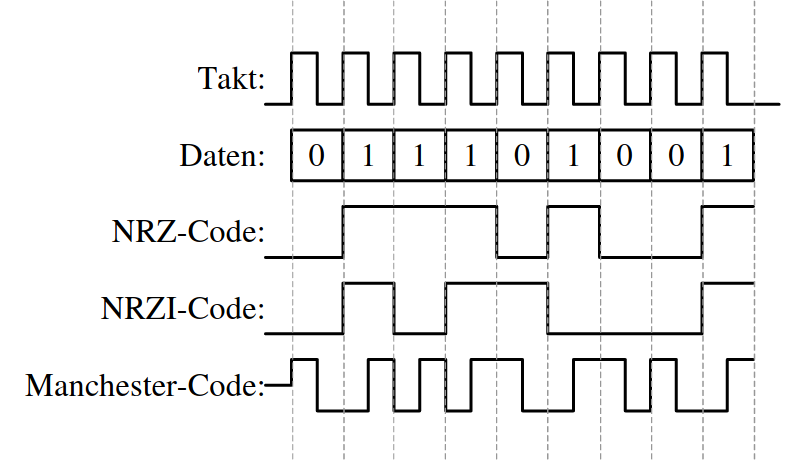
\includegraphics[width=\textwidth]{img/vorlesung12_uebungsaufgabe1_loesung}


\end{document}
